%!TEX root = ../thesis.tex

\chapter[Differential cross section measurement]{Differential cross section measurement}
\label{c:xsection_analysis}
\ifpdf
    \graphicspath{{06_Cross_section_analysis/plots/}}
\else
    \graphicspath{{06_Cross_section_analysis/plots/EPS/}{06_Cross_section_analysis/plots/}}
\fi

% ------------------------------------------------------------------------
Measurement of the differential cross section of the top quark pairs with respect to different variables is an important
precision measurement, but it can also give hints of new physics. For example, measurement of the missing energy in
\ttbar events can represent a search for invisible particles produced in association with top quarks.

The analysis presented in this chapter represents the top quark differential cross section measurement with respect to
event-level (or global) distributions, including the missing transverse energy, the scalar sum of jet transverse momenta
($H_T$) and other variables \autocite{xsection_PAS_7TeV, xsection_PAS_8TeV}. This measurement is used to validate
different Monte Carlo models and generator tunes. Moreover, it provides a sensitive probe for new physics: for instance,
deviations in the tail of the missing transverse energy distribution could signal new resonances with invisible
particles in the final state.

\section{Data and Simulation}
\label{s_xsection:data_and_simulation}

\subsection{Data}
\label{ss_xsection:data}
This analysis uses the full 2012 dataset collected by the CMS detector at a centre of mass energy of \SI{8}{\TeV}, with
a total integrated luminosity of \SI{19.7}{\fbinv}. Only certified events were used in the data, i.e.\ from such
preriods of data-taking when all of the detector subsystems were functioning with no errors. Depending on the channel,
the data were preselected with the single electron or single muon trigger. The preselection procedure as well as full
event selection will be described in Section~\ref{s_xsection:event_selection}.

\subsection{Monte Carlo samples}
\label{ss_xsection:MC_samples}
The Monte Carlo generators used in this work were presented in Section~\ref{sss_top_mass:MC_generators}. The list of
signal and background MC samples is shown in Table~\ref{tab:xsection_mc_samples}, and is largely similar to that from
the top quark mass analysis. In addition, the signal \ttjets sample is also available with \POWHEG and \MCATNLO
generators in order to be able to differentiate between them. Moreover, to extend the statistics of the \W/\ZpJets
samples, they were generated in four exclusive jet multiplicity bins: \W/\Z boson plus one/two/three and at least four
jets.

Table~\ref{tab:xsection_electron_qcd_samples} presents the list of QCD multi-jet background and $\gamma$ + jets samples
used in the estimation of the QCD background in the electron plus jets channel. The analogous set of muon-enriched QCD
samples used in the muon plus jets channel is shown in Table~\ref{tab:xsection_muon_qcd_samples}. Although the QCD
background is estimated using data-driven techniques in both channels (see Section~\ref{s_xsection:data_driven_QCD}),
the MC simulation is still used for normalisation purposes.
% Mention the systematic samples (Table~\ref{tab:xsection_systematic_samples})

\begin{table}[!htbp]
\centering
\caption{Signal and background Monte Carlo samples with cross sections at $\sqrt s =
\SI{8}{\TeV}$, numbers of generated events and corresponding integrated
luminosities.}
\label{tab:xsection_mc_samples}
\begin{tabular}{|l|l|r|r|r|}
\toprule
Process & Generator & $\sigma$ (\pb) & \# events & $\int\lumi dt$ (\fbinv)\\
\midrule
\ttjets, \mtop = \SI{172.5}{\GeV} & \MADGRAPH & 245.8 & 6854416 & 27.9\\
\ttjets, \mtop = \SI{172.5}{\GeV} & \POWHEG  & 245.8 & 21675970 & 88.2\\
\ttjets, \mtop = \SI{172.5}{\GeV} & \MCATNLO & 245.8 & 32706581 & 133.1\\
\midrule
\WpJets ($\W \rightarrow l\nu$) & \MADGRAPH & & & \\
\hspace{5 mm}\W + 1 jet & & 5400.0 & 23141598 & 4.3 \\
\hspace{5 mm}\W + 2 jet & & 1750.0 & 34044921 & 19.5 \\
\hspace{5 mm}\W + 3 jet & & 519.0 & 15539503 & 29.9 \\
\hspace{5 mm}\W + 4 jet & & 214.0 & 13349346 & 62.4 \\
\midrule
$\Z/\gamma^* \rightarrow l^+l^- $ + jets, $m(ll) > \SI{50}{\GeV}$ & \MADGRAPH & & & \\
\hspace{5 mm}\Z + 1 jet & & 561.0 & 24045248 & 42.9 \\
\hspace{5 mm}\Z + 2 jet & & 181.0 & 21852156 & 120.7 \\
\hspace{5 mm}\Z + 3 jet & & 51.1 & 11015445 & 215.6 \\
\hspace{5 mm}\Z + 4 jet & & 23.04 & 6402827 & 277.9 \\
\midrule
Single top & \POWHEG & & & \\
\hspace{5 mm} top t-channel & & 55.5 & 3758227 & 67.7 \\
\hspace{5 mm} anti-top t-channel & & 30.0 & 1935072 & 64.5 \\
\hspace{5 mm} top s-channel & & 3.89 & 259961 & 66.8 \\
\hspace{5 mm} anti-top s-channel & & 1.76 & 139974 & 79.5 \\
\hspace{5 mm} top tW-channel & & 11.18 & 497658 & 44.5 \\
\hspace{5 mm} anti-top tW-channel & & 11.18 & 493460 & 44.1 \\
\bottomrule
\end{tabular}
\end{table}

\begin{table}[!htbp] 
\centering
\caption{QCD multi-jet background and $\gamma$ + jets MC samples used in the electron plus jets channel
with cross sections at $\sqrt s = \SI{8}{\TeV}$, numbers of generated events and corresponding integrated luminosities.
% EM-enriched samples are preselected to include jets with higher electromagnetic content;
% $\cPqb/\cPqc \rightarrow e\nu$ samples are preselected to include leptonic ($e\nu$) in-flight decays of b- and c-quarks.
}
\label{tab:xsection_electron_qcd_samples}
\resizebox{\textwidth}{!}{
\begin{tabular}{|l|l|r|r|r|r|}
\toprule
Process & Generator & $\sigma$ (\pb) & filter efficiency & \# events & $\int\lumi dt$ (\fbinv)\\
\midrule
QCD ($e/\gamma$ enriched)  & \PYTHIA & & & & \\
\hspace{5 mm}\SIrange[range-phrase = $~<\pthat<~$]{20}{30}{\GeV} 	& & \num{2.886d8} 	& \num{1.01d-2} & 34339883 & \num{1.2d-2} \\
\hspace{5 mm}\SIrange[range-phrase = $~<\pthat<~$]{30}{80}{\GeV} 	& & \num{7.433d7} 	& \num{6.21d-2} & 32537408 & \num{7.0d-3} \\
\hspace{5 mm}\SIrange[range-phrase = $~<\pthat<~$]{80}{170}{\GeV} 	& & \num{1.191d6}  	& \num{0.154} &  34542763 & \num{0.19} \\
\hspace{5 mm}\SIrange[range-phrase = $~<\pthat<~$]{170}{250}{\GeV} 	& & \num{30990.0} 	& \num{0.148} & 22862259 & \num{5.0} \\
\hspace{5 mm}\SIrange[range-phrase = $~<\pthat<~$]{250}{350}{\GeV} 	& & \num{4250.0} 	& \num{0.131} &  32505856 & \num{58.4} \\
\hspace{5 mm}$\pthat >$ \SI{350}{\GeV}  							& &	\num{810.0}  	& \num{0.11} &  33981105 & \num{381.4} \\
\midrule
QCD ($\cPqb/\cPqc \rightarrow e\nu$) & \PYTHIA & & & & \\
\hspace{5 mm}\SIrange[range-phrase = $~<\pthat<~$]{20}{30}{\GeV} 	& & \num{2.886d8} 	& \num{5.8d-4} & 1740229 & \num{1.0d-2} \\
\hspace{5 mm}\SIrange[range-phrase = $~<\pthat<~$]{30}{80}{\GeV} 	& & \num{7.433d7} 	& \num{2.25d-3} & 2048152 & \num{1.2d-2} \\
\hspace{5 mm}\SIrange[range-phrase = $~<\pthat<~$]{80}{170}{\GeV} 	& & \num{1.191d6}  	& \num{1.09d-2} & 1945525 & \num{0.15} \\
\hspace{5 mm}\SIrange[range-phrase = $~<\pthat<~$]{170}{250}{\GeV} 	& & \num{30990.0} 	& \num{2.04d-2} & 1948112 & \num{3.1} \\
\hspace{5 mm}\SIrange[range-phrase = $~<\pthat<~$]{250}{350}{\GeV} 	& & \num{4250.0}  	& \num{2.43d-2} & 2026521 & \num{19.6} \\
\hspace{5 mm}$\pthat >$ \SI{350}{\GeV} 								& &	\num{810.0}  	& \num{2.95d-2} & 1948532 & \num{81.5} \\
\midrule
$\gamma$ + jets & \MADGRAPH & & & & \\
\hspace{5 mm}\SIrange[range-phrase = $~<\HT<~$]{200}{400}{\GeV} & & \num{960.5} & 1 & 10479625 & \num{10.9} \\
\hspace{5 mm}$\HT >$ \SI{400}{\GeV} & & \num{107.5} & 1 & 1611963 & \num{15.0} \\
\bottomrule
\end{tabular}
}
\end{table}

\begin{table}[!htbp] 
\centering
\caption{QCD multi-jet background MC samples used in the muon plus jets channel with cross sections at $\sqrt s =
\SI{8}{\TeV}$, numbers of generated events and corresponding integrated luminosities.}
\label{tab:xsection_muon_qcd_samples}
\resizebox{\textwidth}{!}{
\begin{tabular}{|l|l|r|r|r|r|}
\toprule
Process & Generator & $\sigma$ (\pb) & filter efficiency & \# events & $\int\lumi dt$ (\fbinv)\\
\midrule
QCD ($\mu$ enriched)  & \PYTHIA & & & & \\
\hspace{5 mm}\SIrange[range-phrase = $~<\pthat<~$]{15}{20}{\GeV} 	& & \num{7.022d8} 	& \num{3.9d-3}	& 1722681	& \num{6.3d-4} \\
\hspace{5 mm}\SIrange[range-phrase = $~<\pthat<~$]{20}{30}{\GeV} 	& & \num{2.87d8} 	& \num{6.5d-3}	& 8486904	& \num{4.5d-3} \\
\hspace{5 mm}\SIrange[range-phrase = $~<\pthat<~$]{30}{50}{\GeV} 	& & \num{6.609d7} 	& \num{1.22d-2}	& 9560265	& \num{1.2d-2} \\
\hspace{5 mm}\SIrange[range-phrase = $~<\pthat<~$]{50}{80}{\GeV} 	& & \num{8.082d6} 	& \num{2.18d-2}	& 10365230	& \num{5.9d-2} \\
\hspace{5 mm}\SIrange[range-phrase = $~<\pthat<~$]{80}{120}{\GeV} 	& & \num{1.024d6}	& \num{3.95d-2}	& 9238642	& \num{0.23} \\
\hspace{5 mm}\SIrange[range-phrase = $~<\pthat<~$]{120}{170}{\GeV} 	& & \num{1.578d5}	& \num{4.73d-2}	& 8501935	& \num{1.1} \\
\hspace{5 mm}\SIrange[range-phrase = $~<\pthat<~$]{170}{300}{\GeV} 	& & \num{34020.0}	& \num{6.76d-2}	& 7669947	& \num{3.3} \\
\hspace{5 mm}\SIrange[range-phrase = $~<\pthat<~$]{300}{470}{\GeV} 	& & \num{1757.0}	& \num{8.64d-2}	& 7832261	& \num{51.6} \\
\hspace{5 mm}\SIrange[range-phrase = $~<\pthat<~$]{470}{600}{\GeV} 	& & \num{115.2}		& \num{0.102}	& 3783069	& \num{322.0} \\
\hspace{5 mm}\SIrange[range-phrase = $~<\pthat<~$]{600}{800}{\GeV} 	& & \num{27.01}		& \num{0.0996}	& 4119000	& \num{1531.1} \\
\hspace{5 mm}\SIrange[range-phrase = $~<\pthat<~$]{800}{1000}{\GeV} & & \num{3.57}		& \num{0.1033}	& 4107853	& \num{11139.0} \\
\hspace{5 mm}$\pthat >$ \SI{1000}{\GeV}  							& &	\num{0.774}		& \num{0.1097}	& 3873970	& \num{45625.6} \\
\bottomrule
\end{tabular}
}
\end{table}

\begin{table}[!htbp]
\centering
\caption{Systematic MC samples with cross sections at $\sqrt s =
\SI{8}{\TeV}$, numbers of generated events and corresponding integrated
luminosities. Factorisation scale $Q$ and matching threshold systematic
uncertainties are estimated with variations of \ttjets, \WpJets and \ZpJets
samples.}
\label{tab:xsection_systematic_samples}
\begin{tabular}{|l|l|r|r|r|}
\toprule
Process & Generator & $\sigma$ (\pb) & \# events & $\int\lumi dt$ (\fbinv)\\
\midrule
\ttjets & \MADGRAPH & & & \\
\hspace{5 mm}$0.5~\times$ matching threshold 	& & 245.8 & 5476728	& 10.2 \\
\hspace{5 mm}$2~\times$ matching threshold  	& & 245.8 & 5306710	& 25.5 \\
\hspace{5 mm}$0.5\times Q$  					& & 245.8 & 5387181 & 25.4 \\
\hspace{5 mm}$2\times Q$ 						& & 245.8 & 5009488 & 23.4 \\
\midrule
\WpJets ($\W \rightarrow l\nu$) & \MADGRAPH & & & \\
\hspace{5 mm}$0.5~\times$ matching threshold 	& & 29690 & 21364637 & 0.7 \\
\hspace{5 mm}$2~\times$ matching threshold 		& & 30290 & 20976082 & 0.7 \\
\hspace{5 mm}$0.5 \times Q$ 					& & 33300 & 20719363 & 0.6 \\
\hspace{5 mm}$2 \times Q$ 						& & 32000 & 20784770 & 0.6 \\
\midrule
\ZpJets ($\Z \rightarrow ll$) & \MADGRAPH & & & \\
\hspace{5 mm}$0.5~\times$ matching threshold 	& & 2888 & 2112387 & 0.6 \\
\hspace{5 mm}$2~\times$ matching threshold 		& & 2915 & 1985529 & 0.7 \\
\hspace{5 mm}$0.5 \times Q$ 					& & 3312 & 1934901 & 0.6 \\
\hspace{5 mm}$2 \times Q$ 						& & 2954 & 2170270 & 0.7 \\
\bottomrule
\end{tabular}
\end{table}

% WARNING: V+Jets systematic samples cross sections are 7 TeV ones (taken from PREP)
% Does this affect the measurement of the systematics?

\subsection{Pile-up reweighting}
\label{sss_xsection:pileup_reweighting}
Since the number of simulated pile-up interactions does not necessarily represent the same distribution in data, a
reweighting procedure for MC events is required. To produce the weights, measured instantaneous luminosity is used to
obtain a distribution of true pile-up vertices in data, i.e.\ before any vertex reconstruction inefficiencies. This
distribution is then divided by the simulated one, and for each number of pile-up interactions, the weight is
calculated. Figure~\ref{fig:pileup_vertices} shows the number of interactions before and after reweighting for both
electron an muon channels. Evidently, the reweighting procedure helps to achieve a good agreement between data and
simulation.

\begin{figure}[!htpb]
\begin{center}
	\subfloat[]{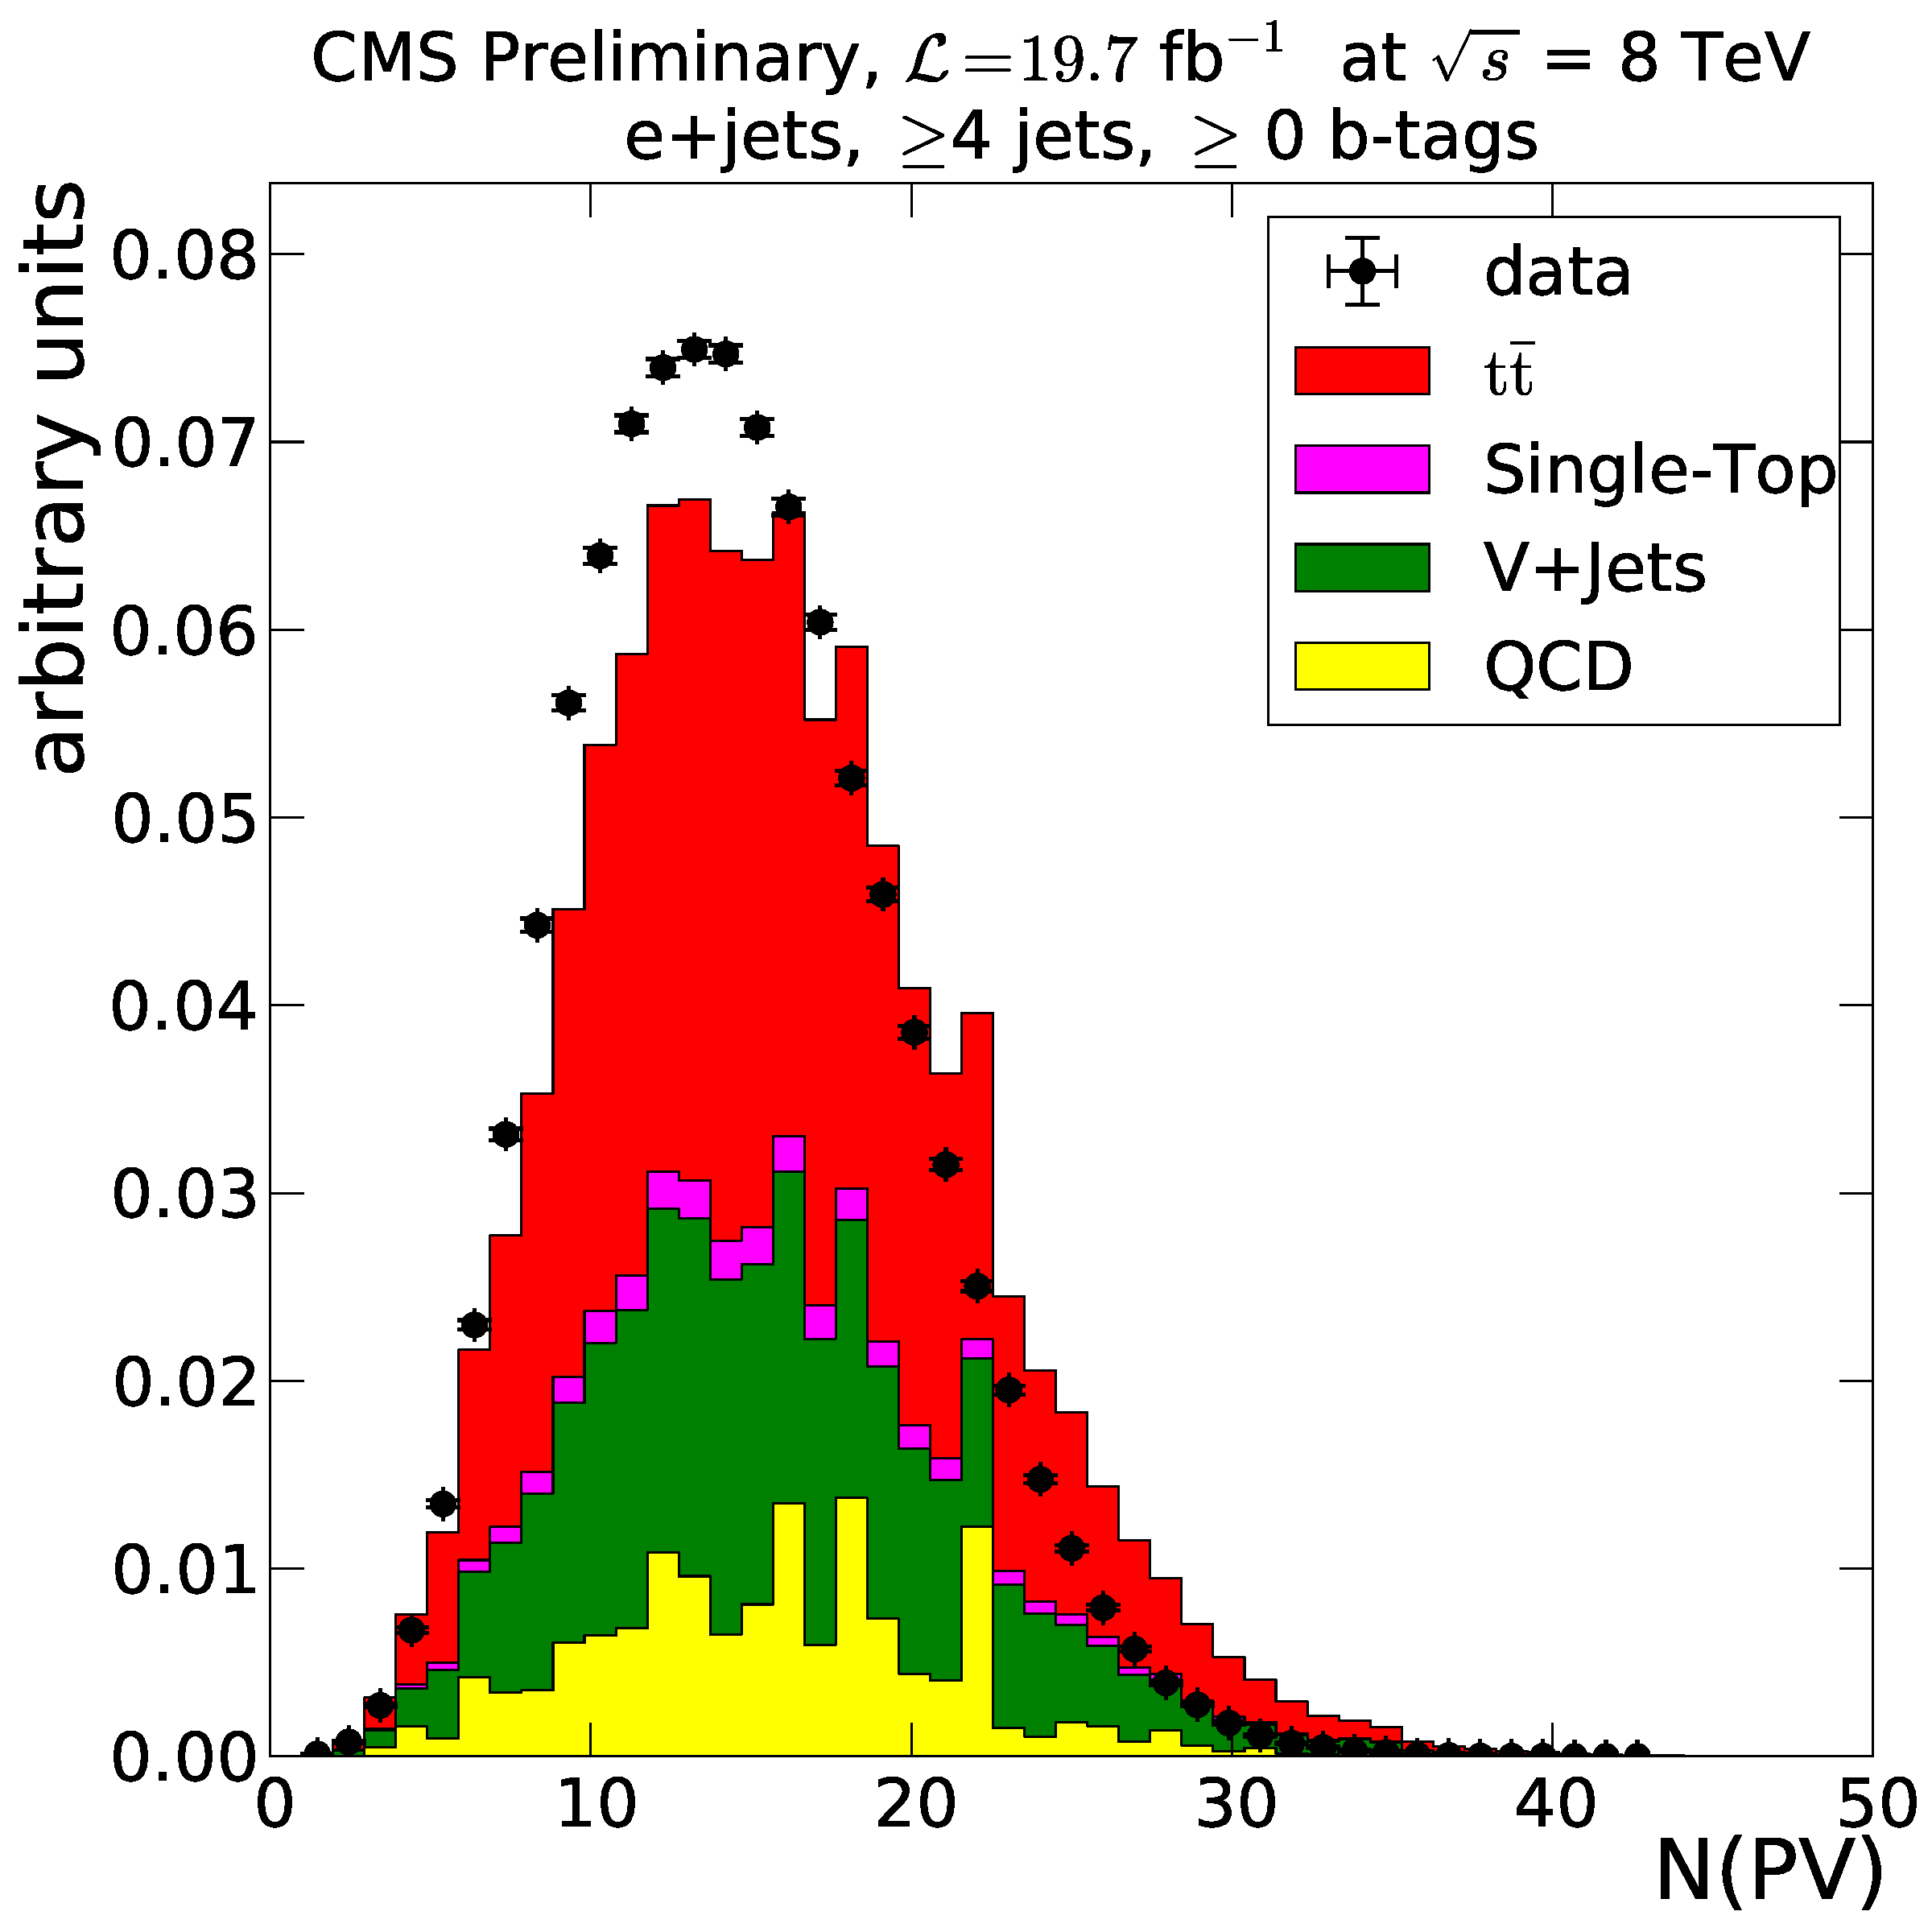
\includegraphics[width=0.50\textwidth]{vertices/EPlusJets_nVertex.pdf}}\hfill
	\subfloat[]{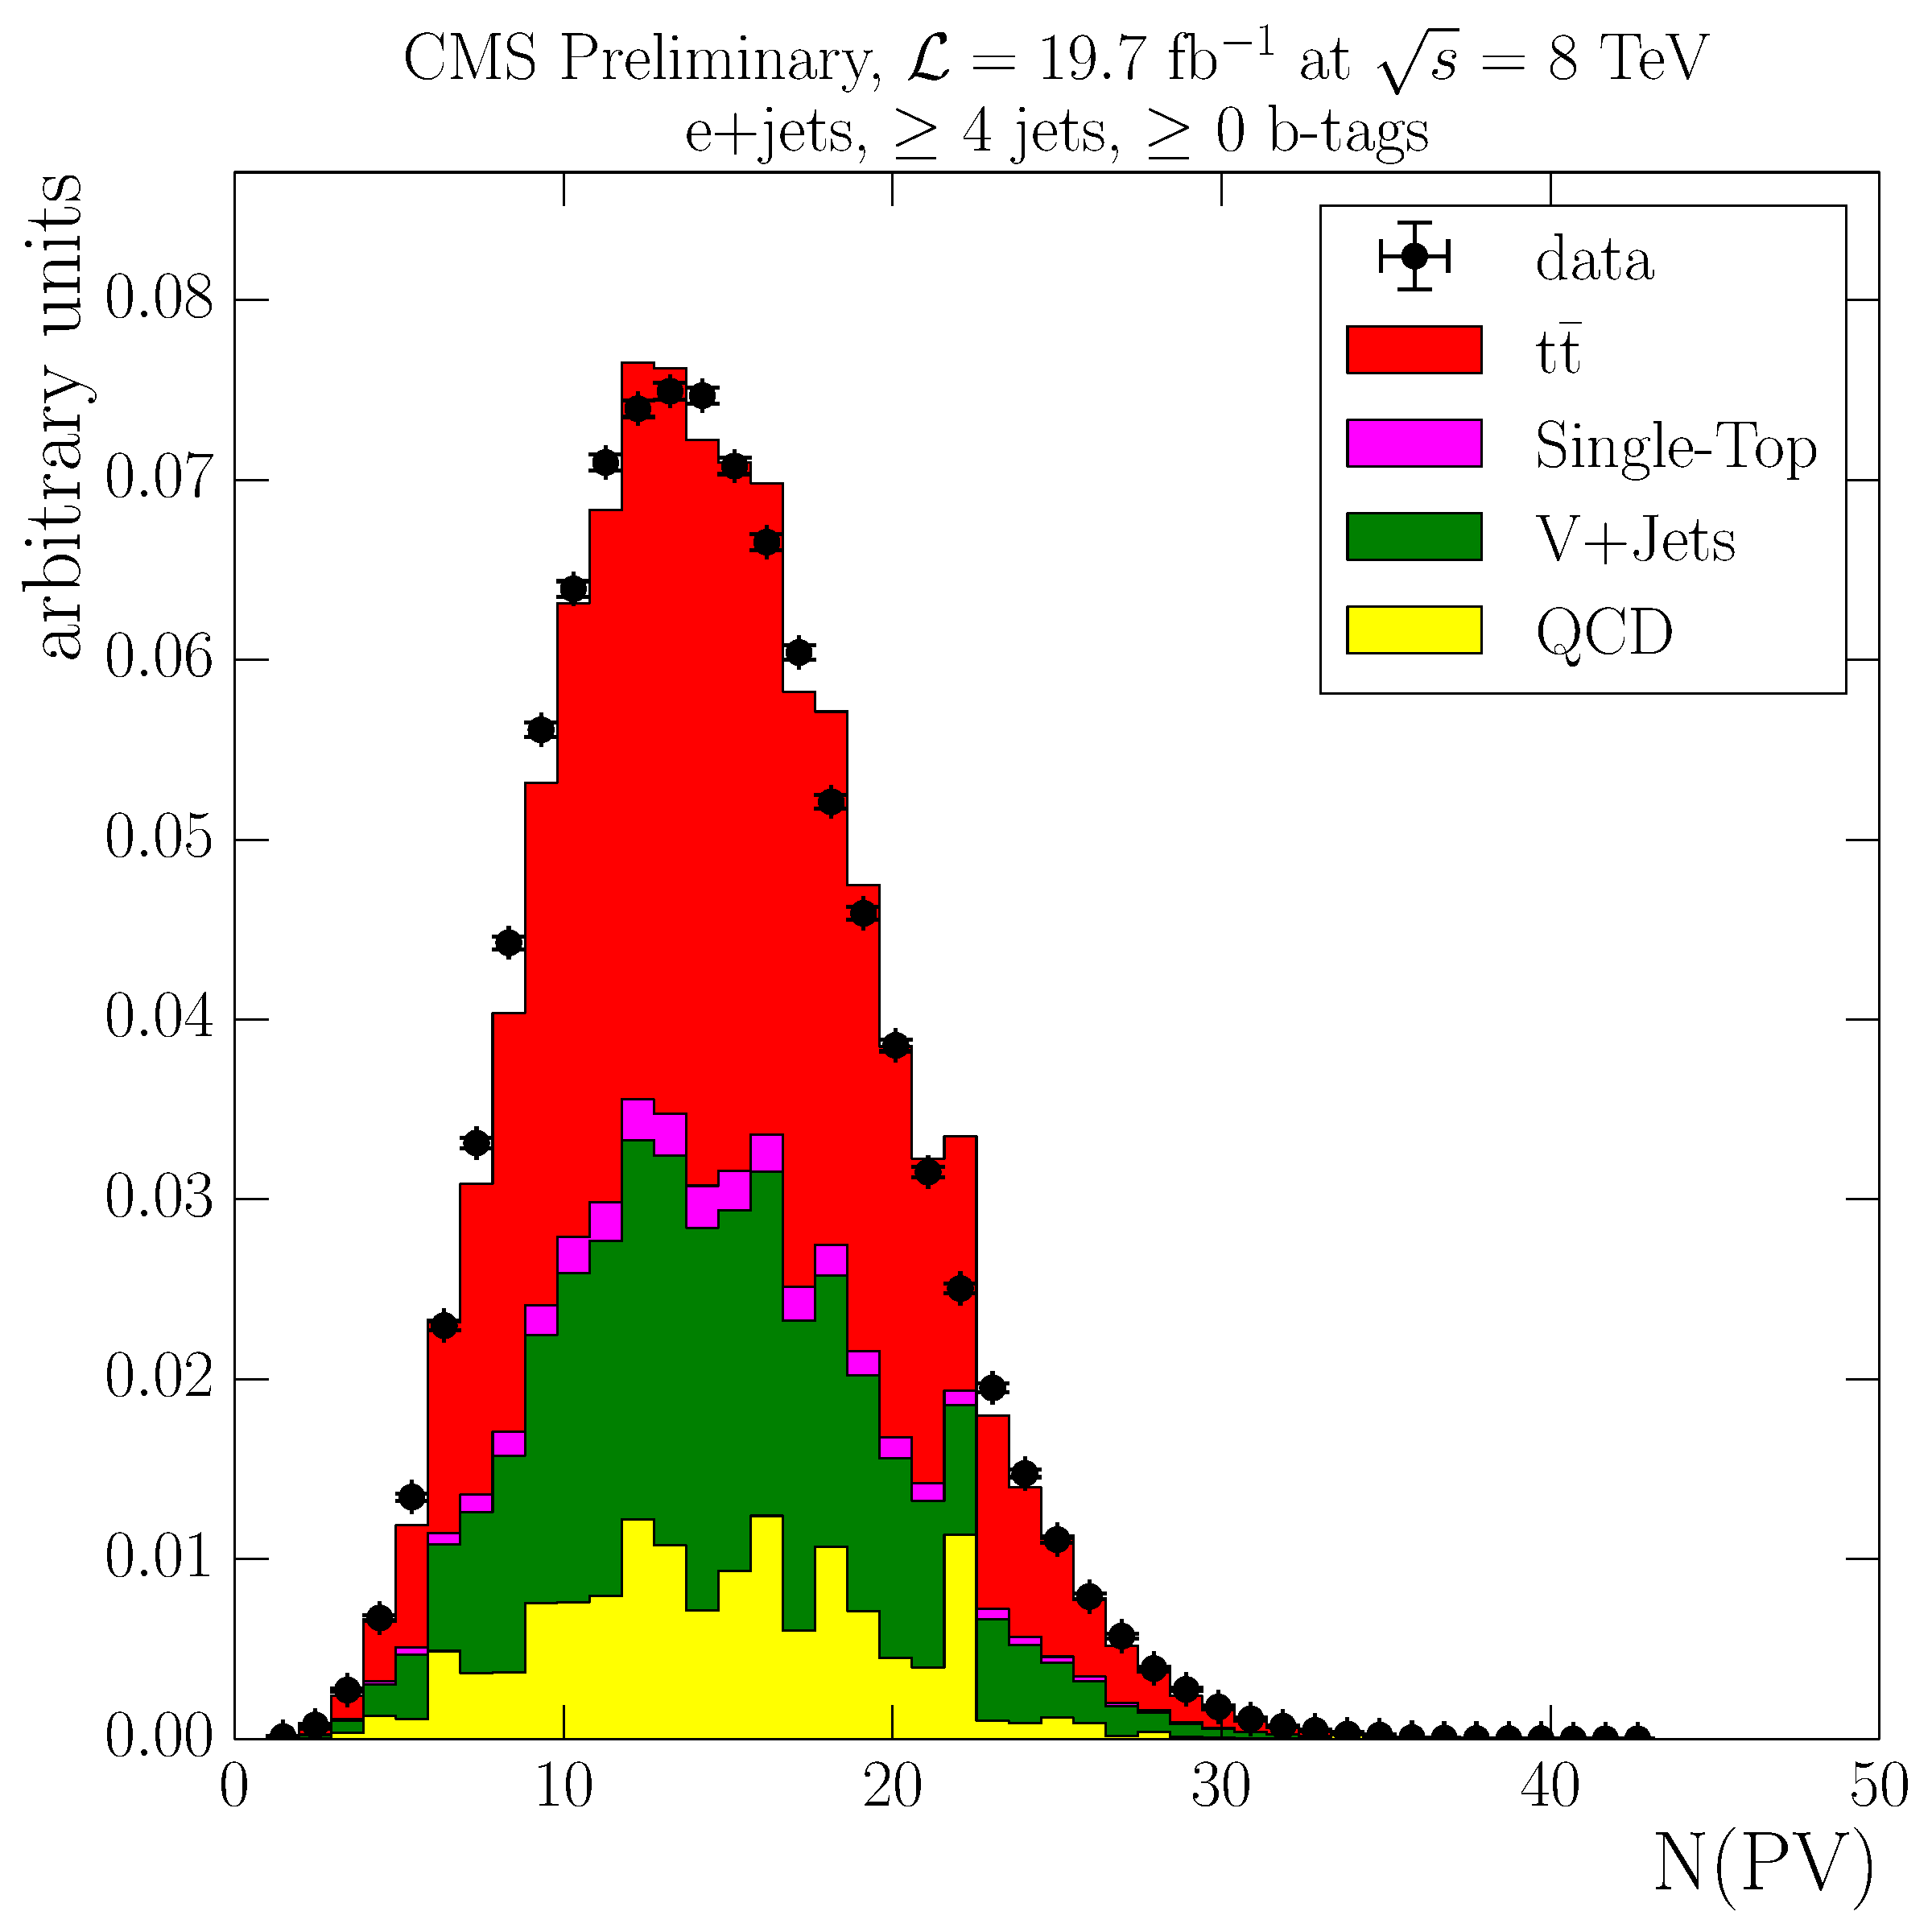
\includegraphics[width=0.50\textwidth]{vertices/EPlusJets_nVertex_reweighted.pdf}} \\
	\subfloat[]{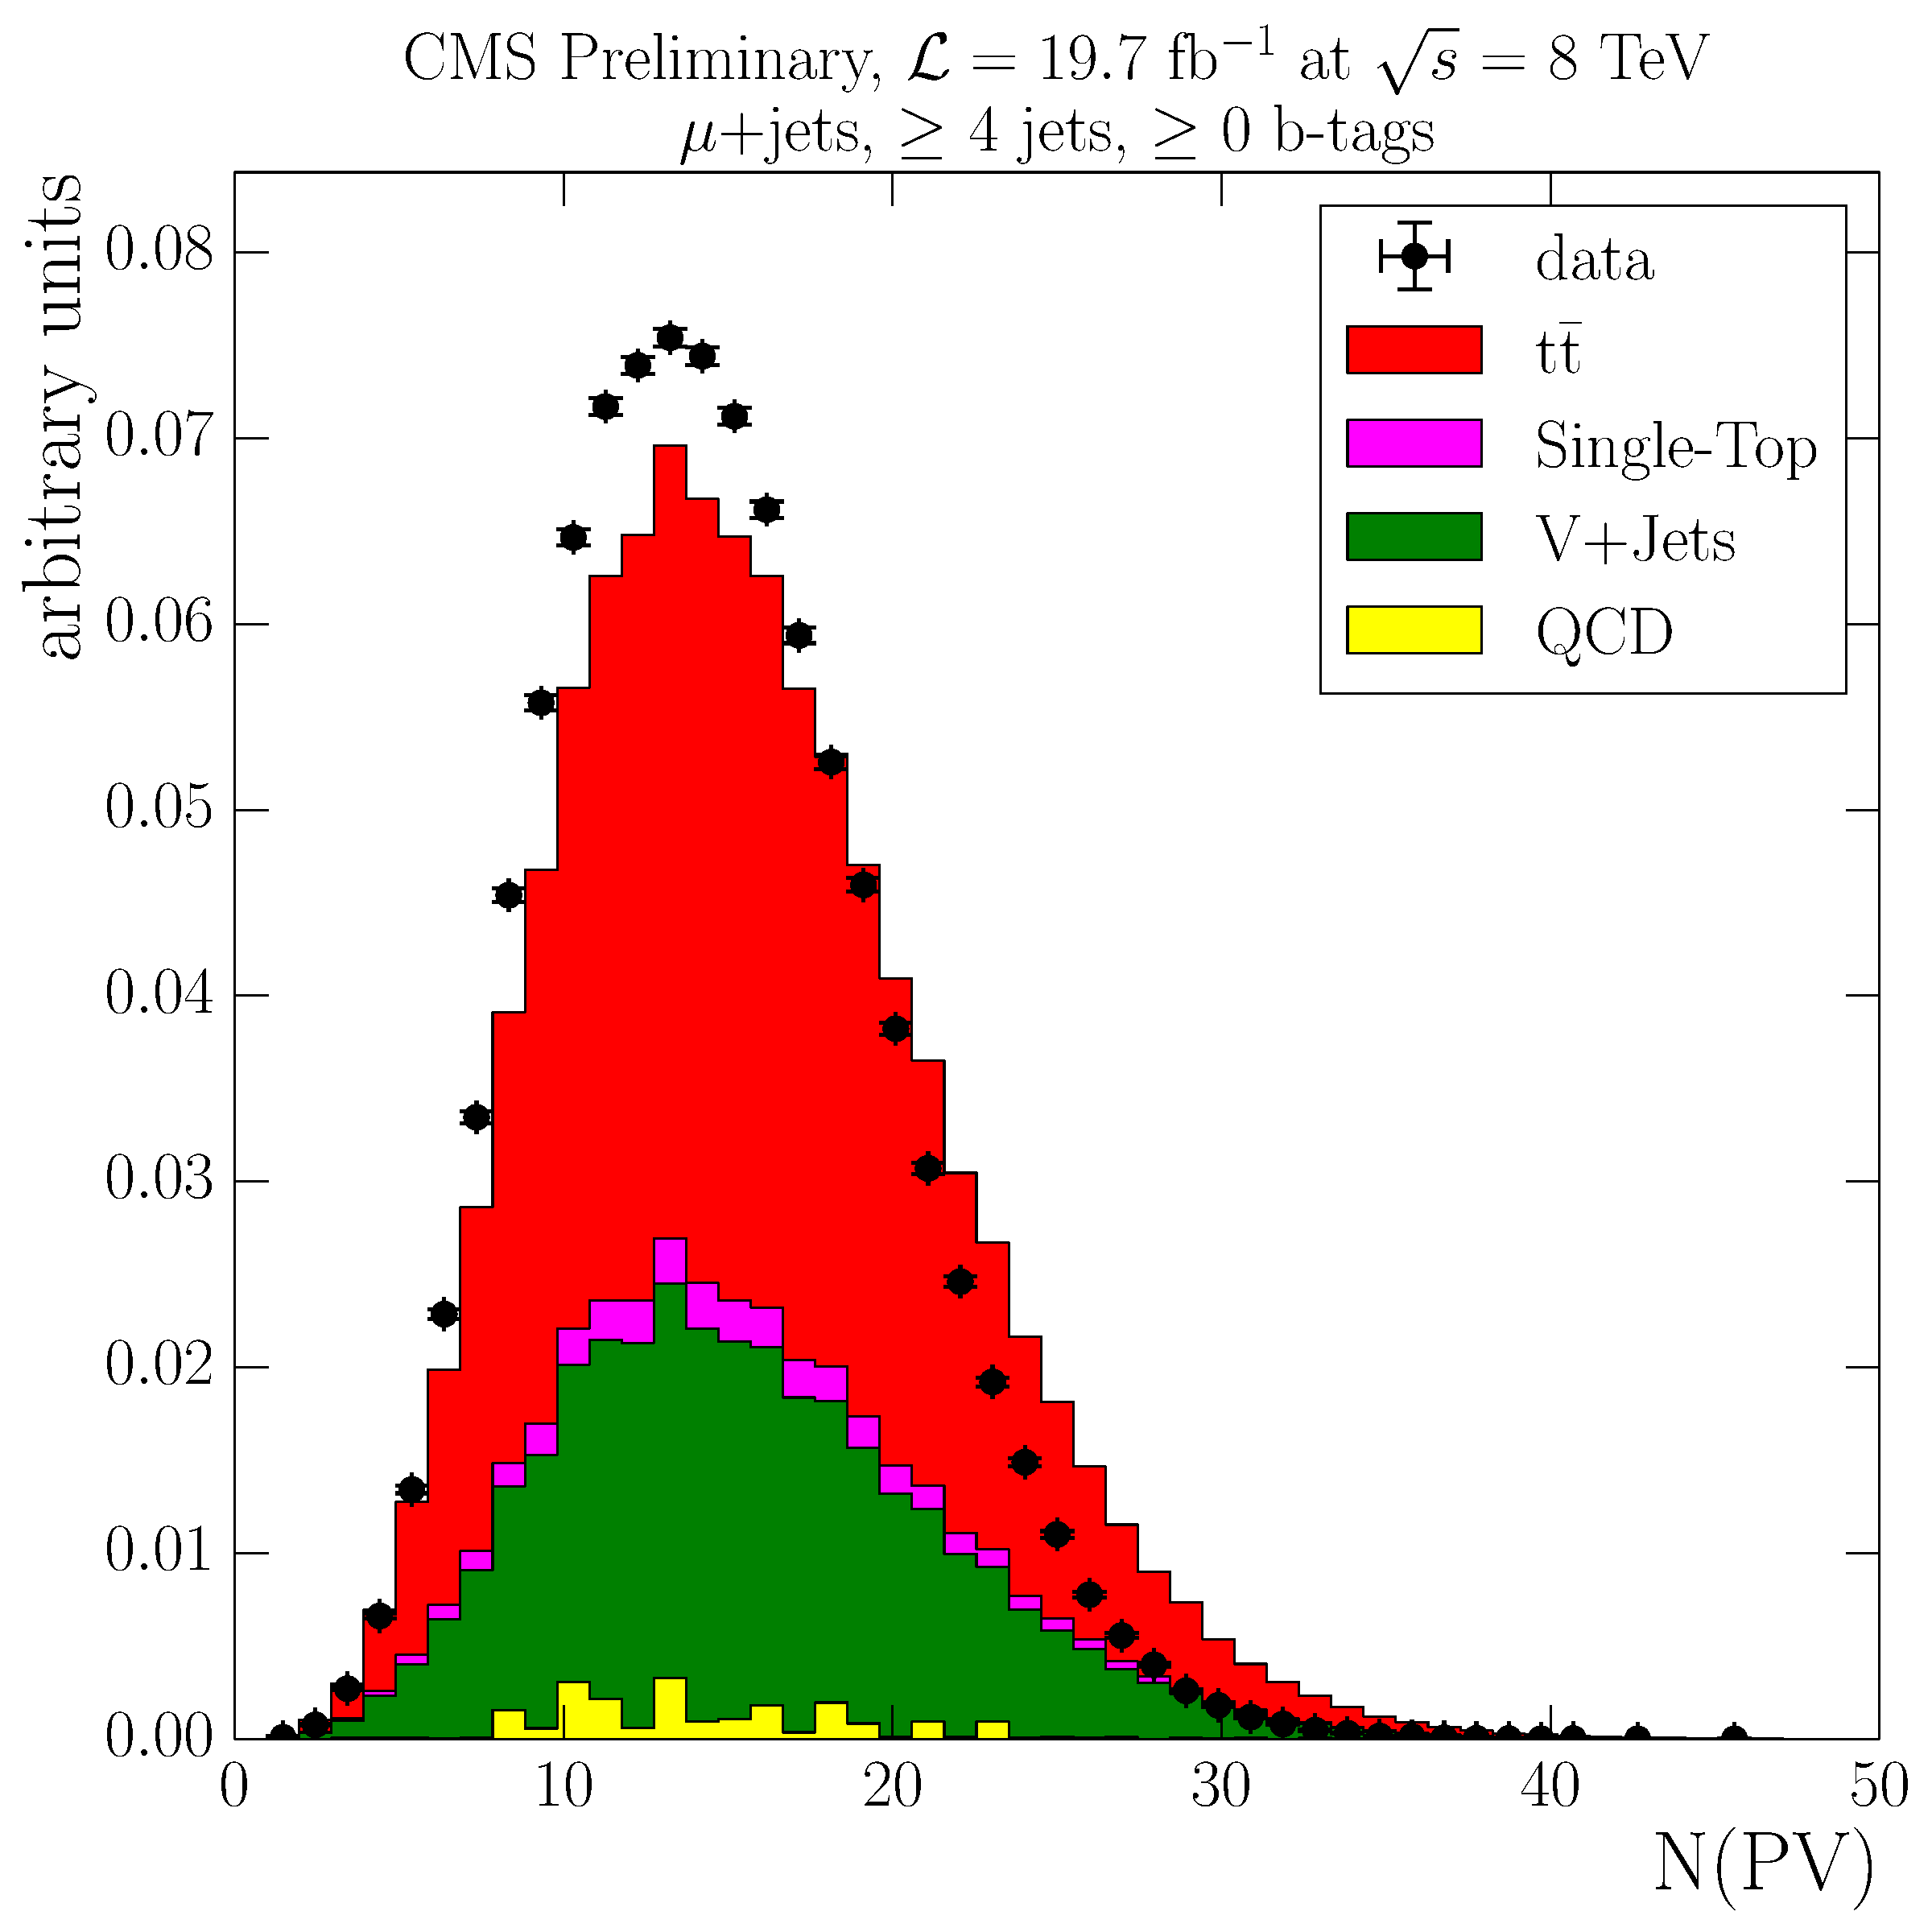
\includegraphics[width=0.50\textwidth]{vertices/MuPlusJets_nVertex.pdf}}\hfill
	\subfloat[]{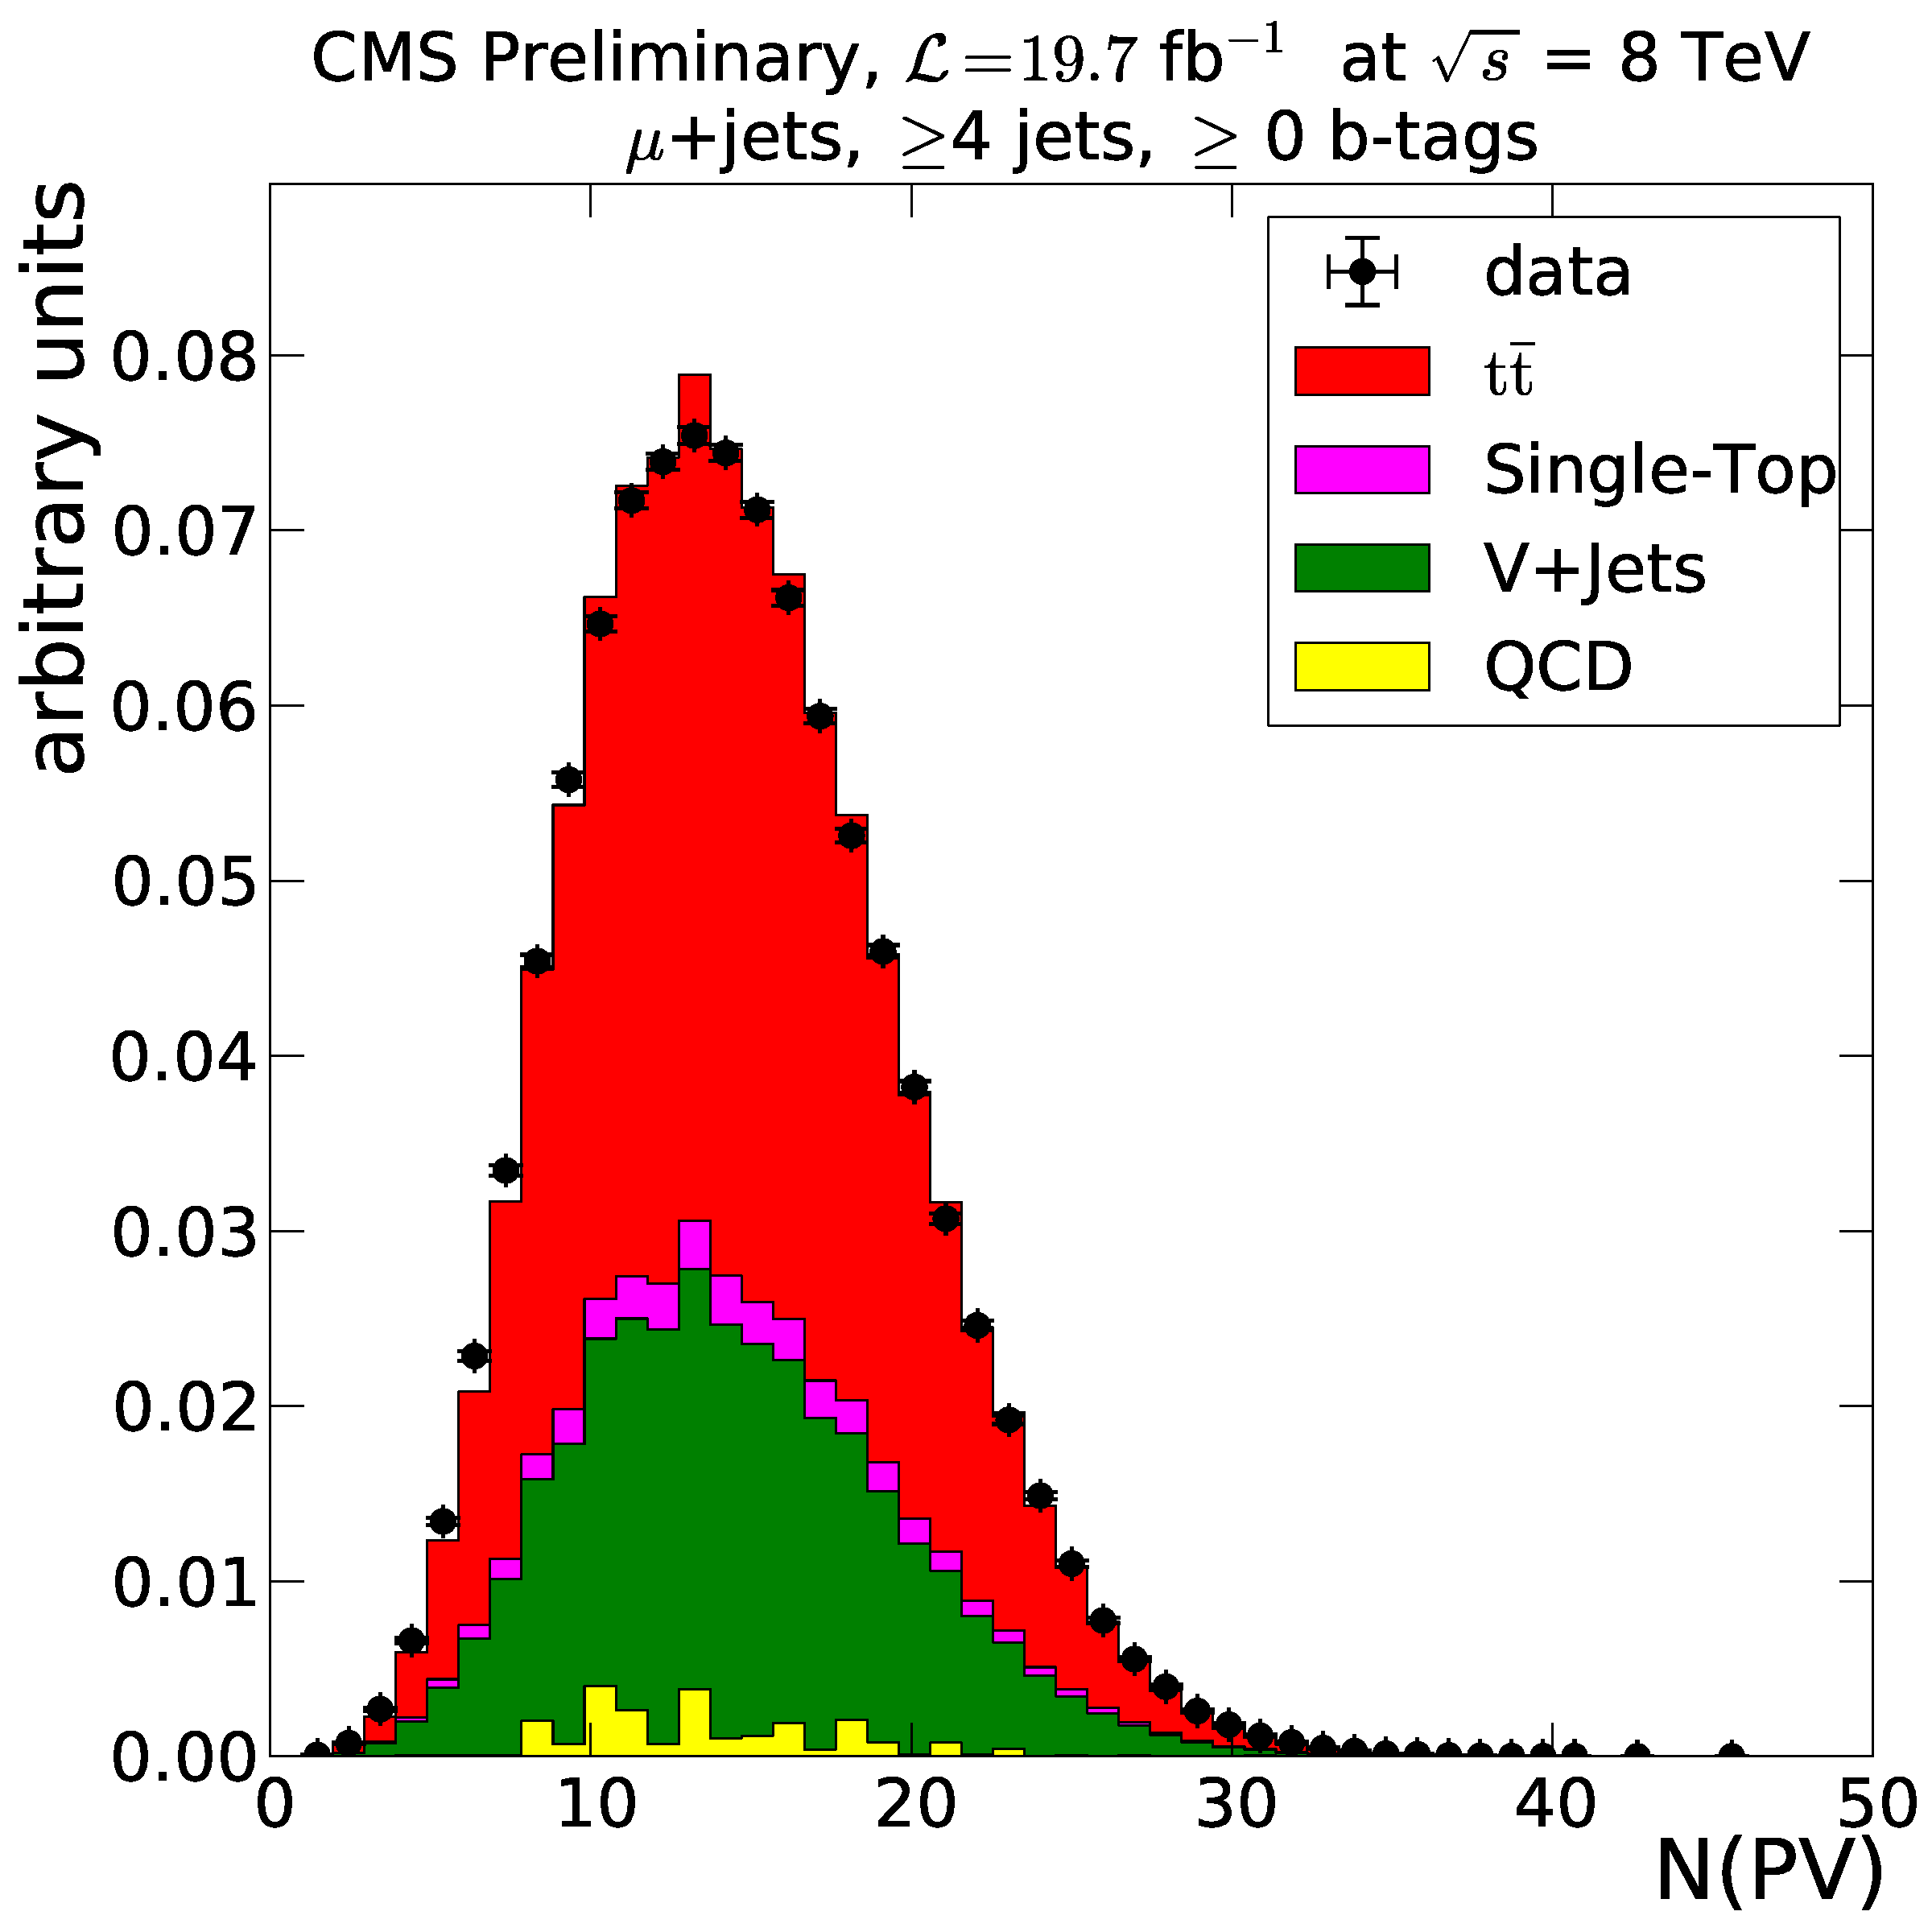
\includegraphics[width=0.50\textwidth]{vertices/MuPlusJets_nVertex_reweighted.pdf}}
	\caption{\label{fig:pileup_vertices}
    Number of reconstructed vertices per event before (left) and after pile-up reweighting (right) in the electron
    channel (top) and in the muon channel (bottom). Both data and sum of the MC samples are normalised to unit area.}
    %QCD is estimated from MC here. Possible to fix/remove?
\end{center}
\end{figure}

To estimate the number of pile-up vertices in data, the measured instantaneous luminosity in each bunch crossing is
multiplied by an average total inelastic proton-proton cross section. Therefore, two sources of uncertainty arise from
these factors: the luminosity uncertainty, measured to be \SI{4.4}{\pc} by a dedicated study \autocite{CMS_lumi_2012},
and the uncertainty on the total inelastic cross section. To obtain the total cross section value, the CMS measurement
of \SI{68\pm4.5}{\milli\barn} based on \SI{7}{\TeV} data \autocite{CMS_total_inelastic_7TeV} was extrapolated to the
\SI{8}{\TeV} value of \SI{69.3}{\milli\barn}. The recommended uncertainty on this value, set to be \SI{5}{\pc}, covers
the modelling and physics aspects of pile-up simulation that have not been fully studied up to date.

%https://twiki.cern.ch/twiki/bin/viewauth/CMS/PileupSystematicErrors (this has been updated to 69.4mb!)

The effect of the \SI{\pm5}{\pc} variations in total inelastic cross section on the estimate of the true number of
vertices in data is shown in Figure~\ref{fig:pileup_truth}, whereas its effect on the simulated distributions is shown
in Figure~\ref{fig:pileup_vertices_variations} for both electron and muon channels.

 \begin{figure}[hbtp]
   \centering
     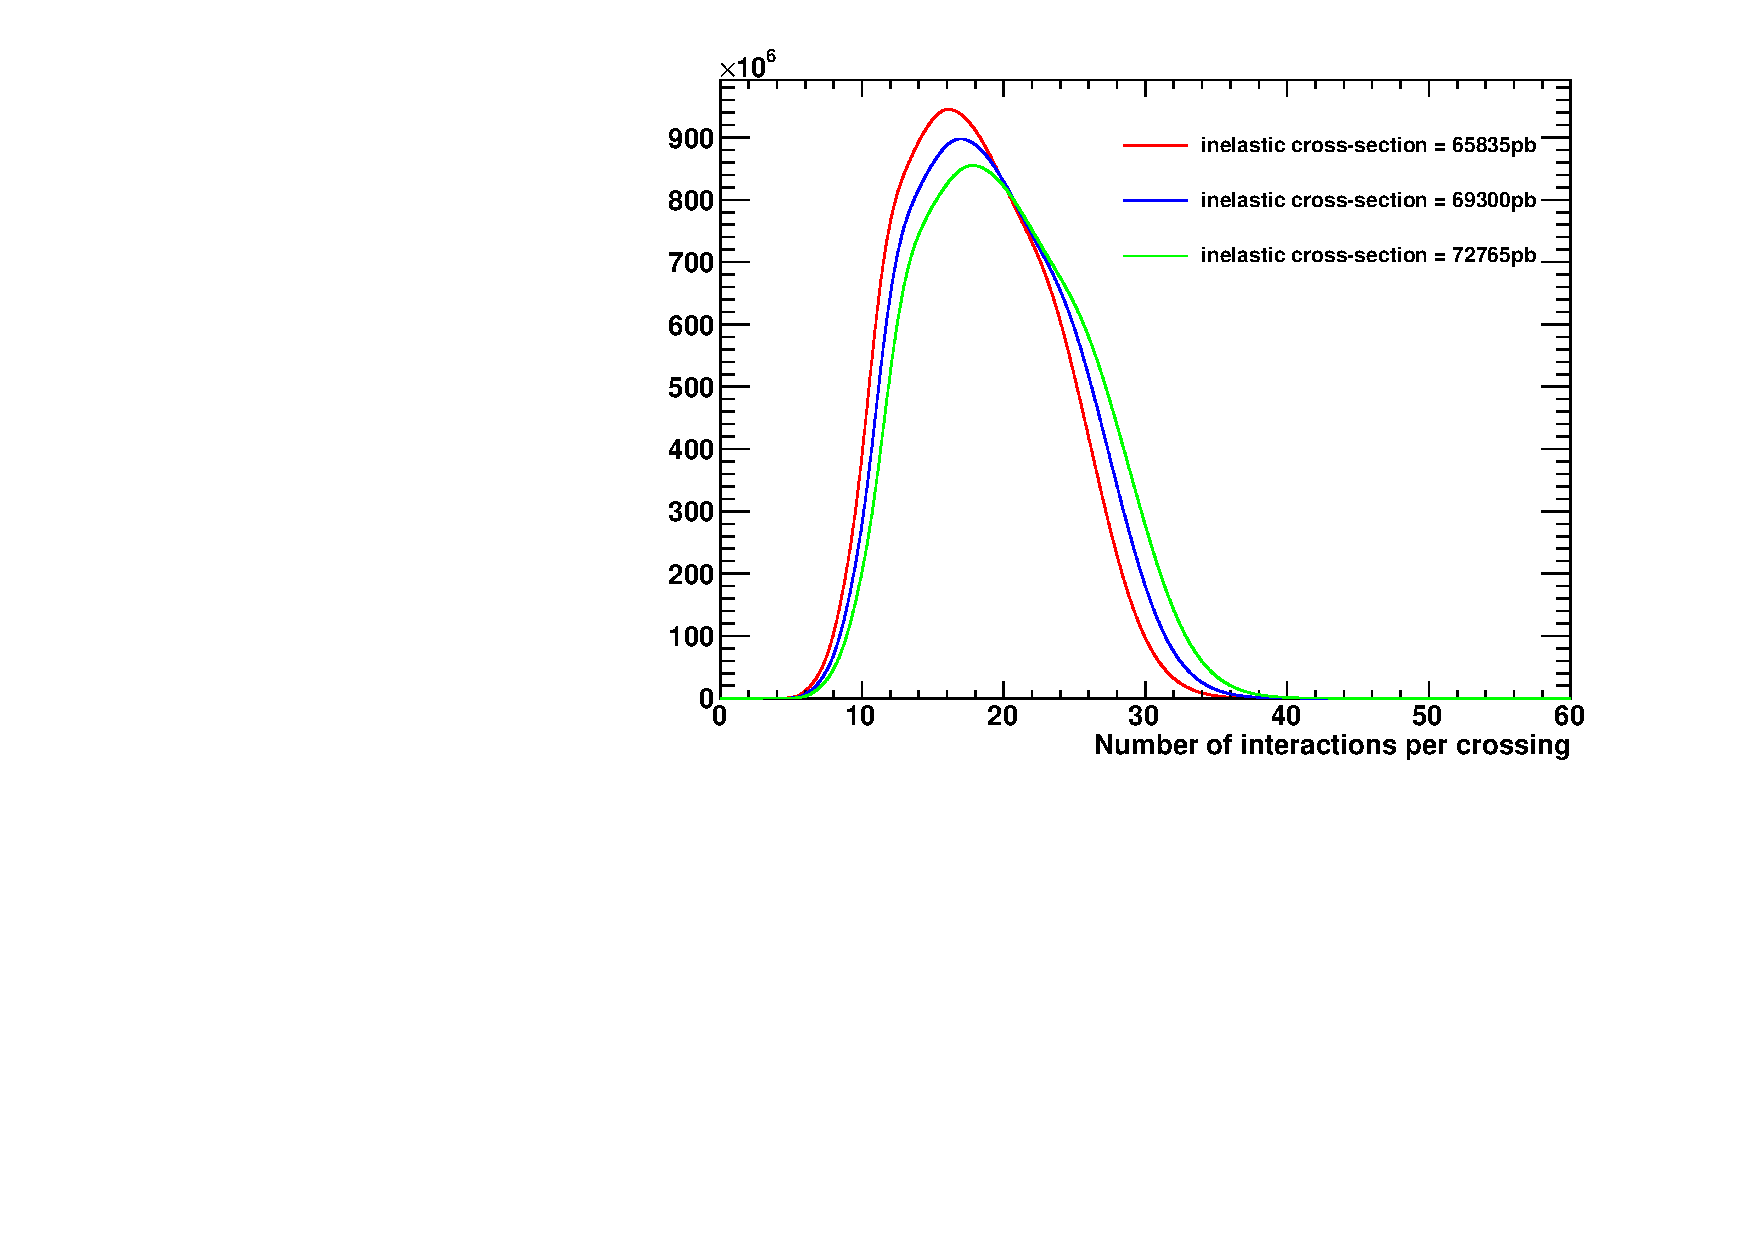
\includegraphics[width=\textwidth]{vertices/PileUp_2012_truth_data.pdf}
     \caption{Number of expected vertices per event for central and $\pm \sigma$ variations of the total inelastic cross
     section for the 2012 data.}
     \label{fig:pileup_truth}
 \end{figure}

\begin{figure}[!htpb]
\begin{center}
	\subfloat[]{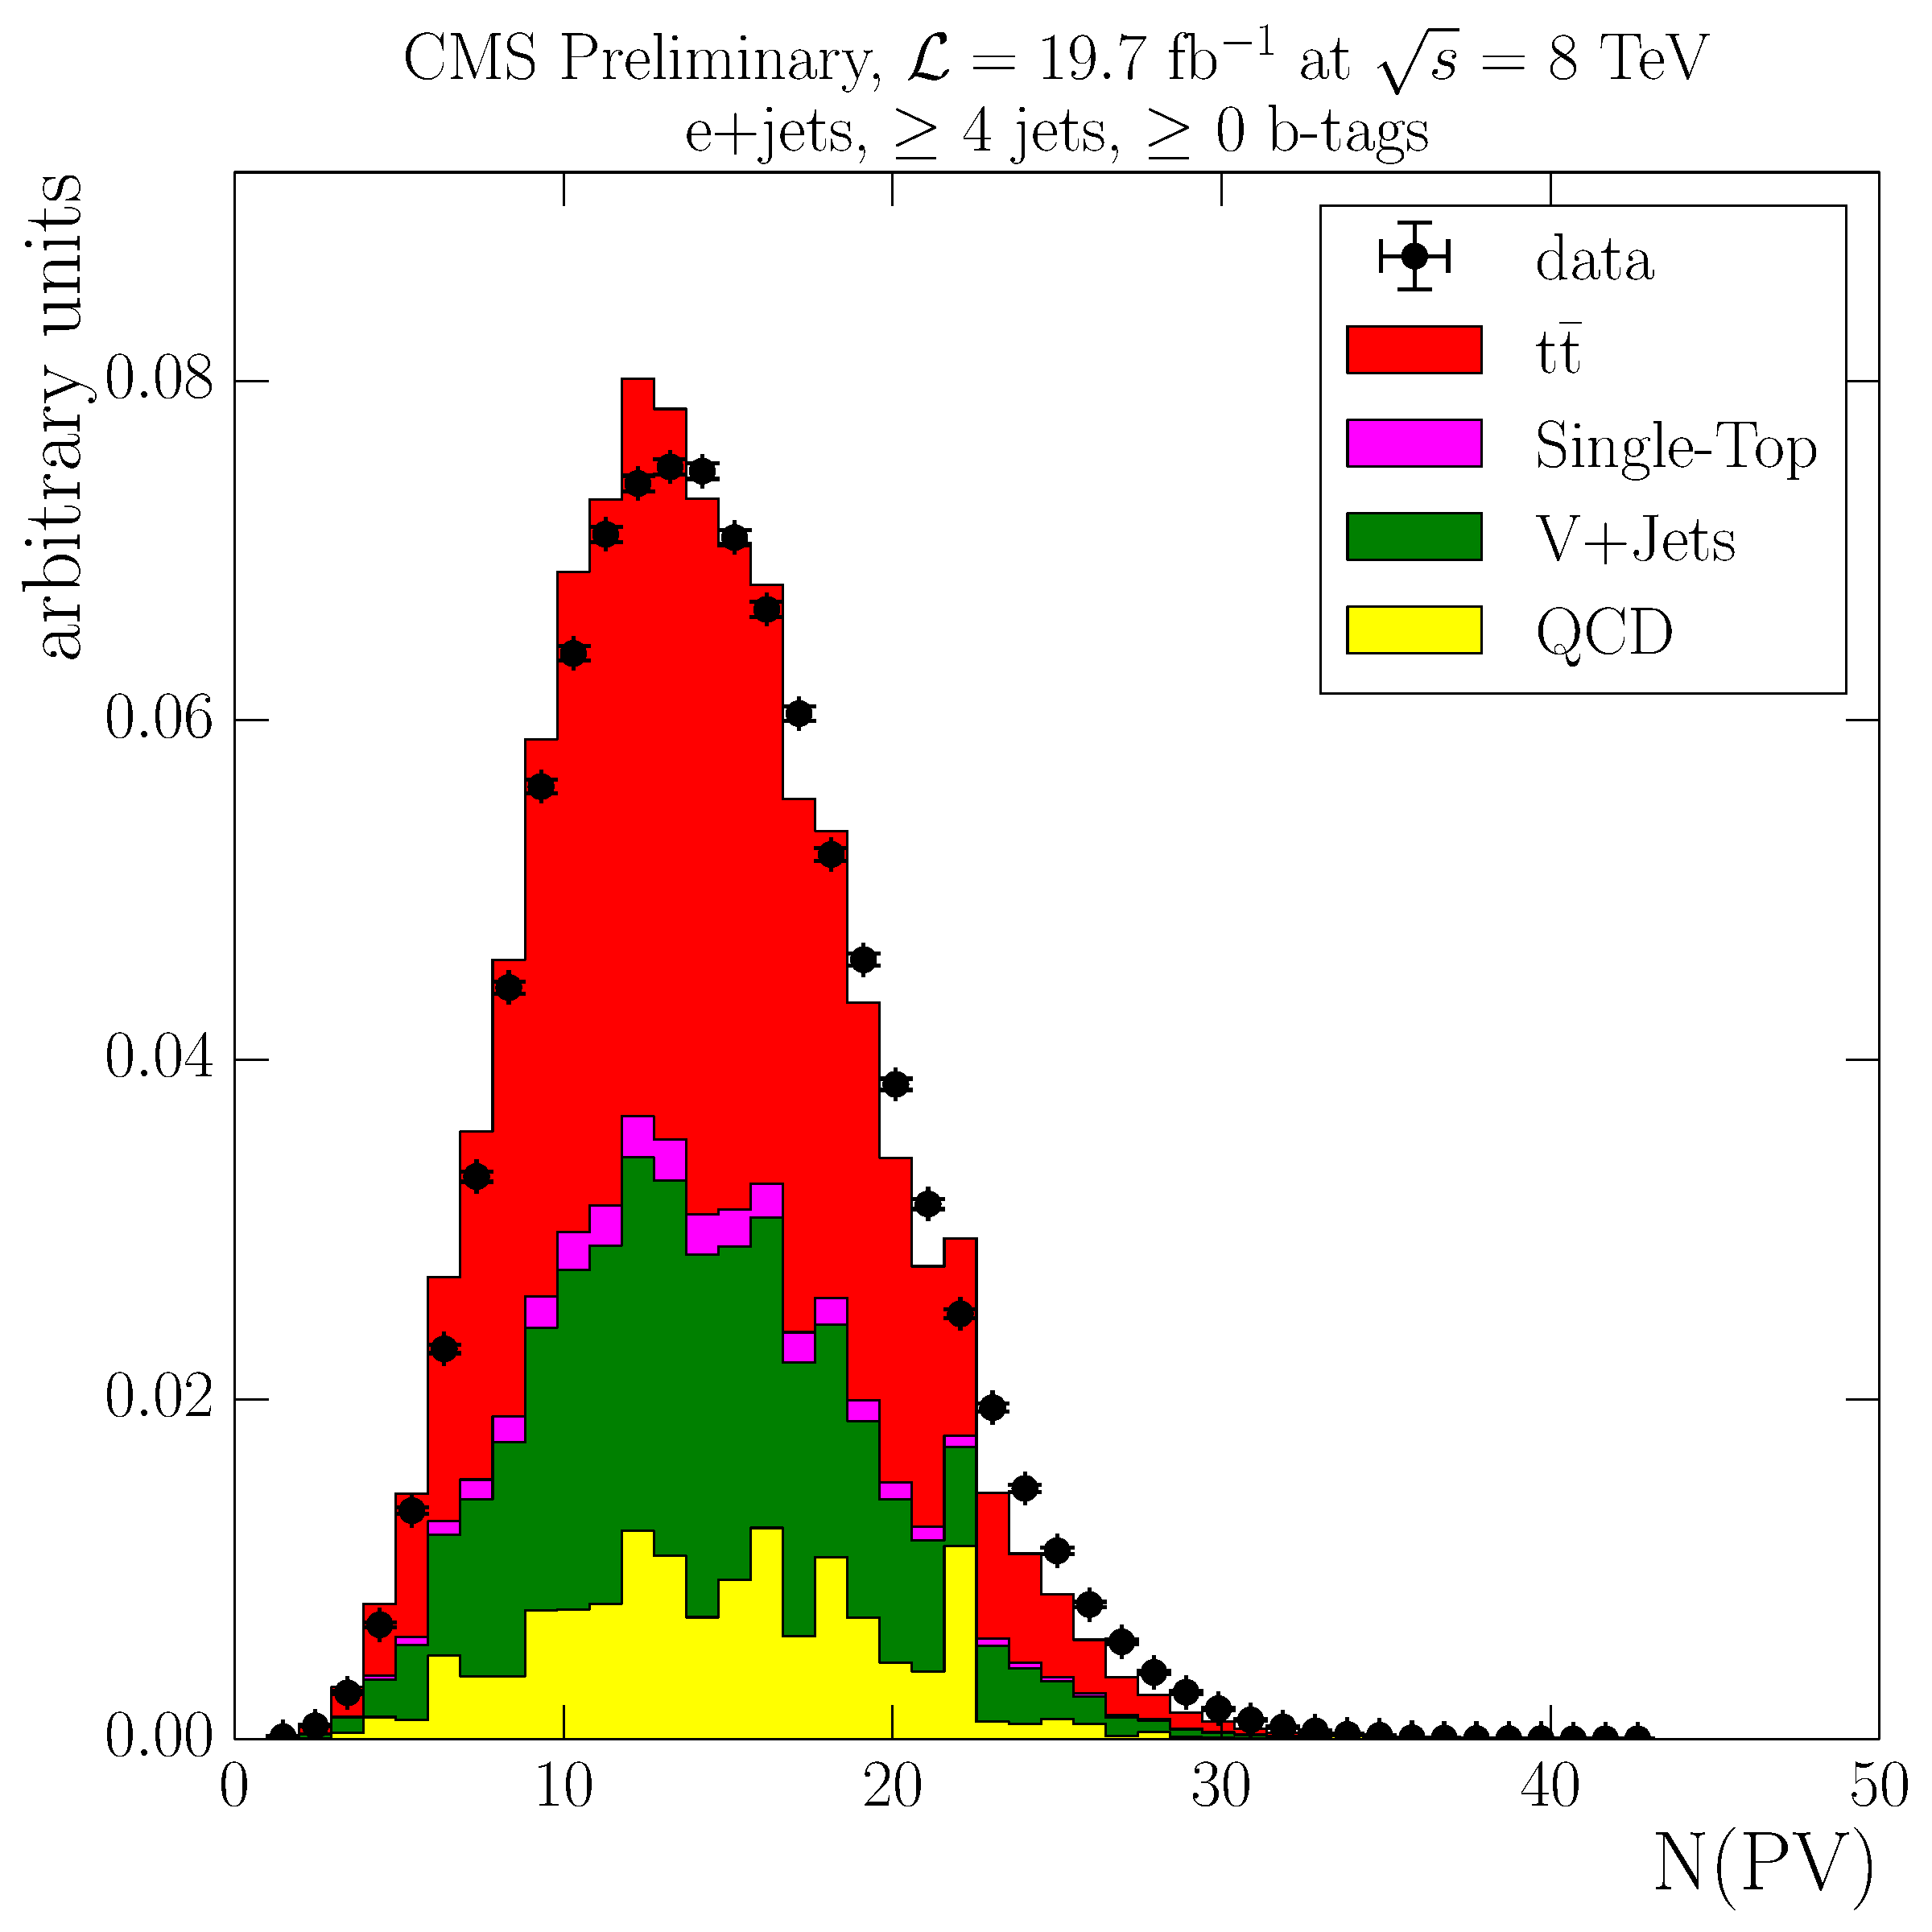
\includegraphics[width=0.50\textwidth]{vertices/EPlusJets_nVertex_reweighted_PU_down.pdf}}\hfill
	\subfloat[]{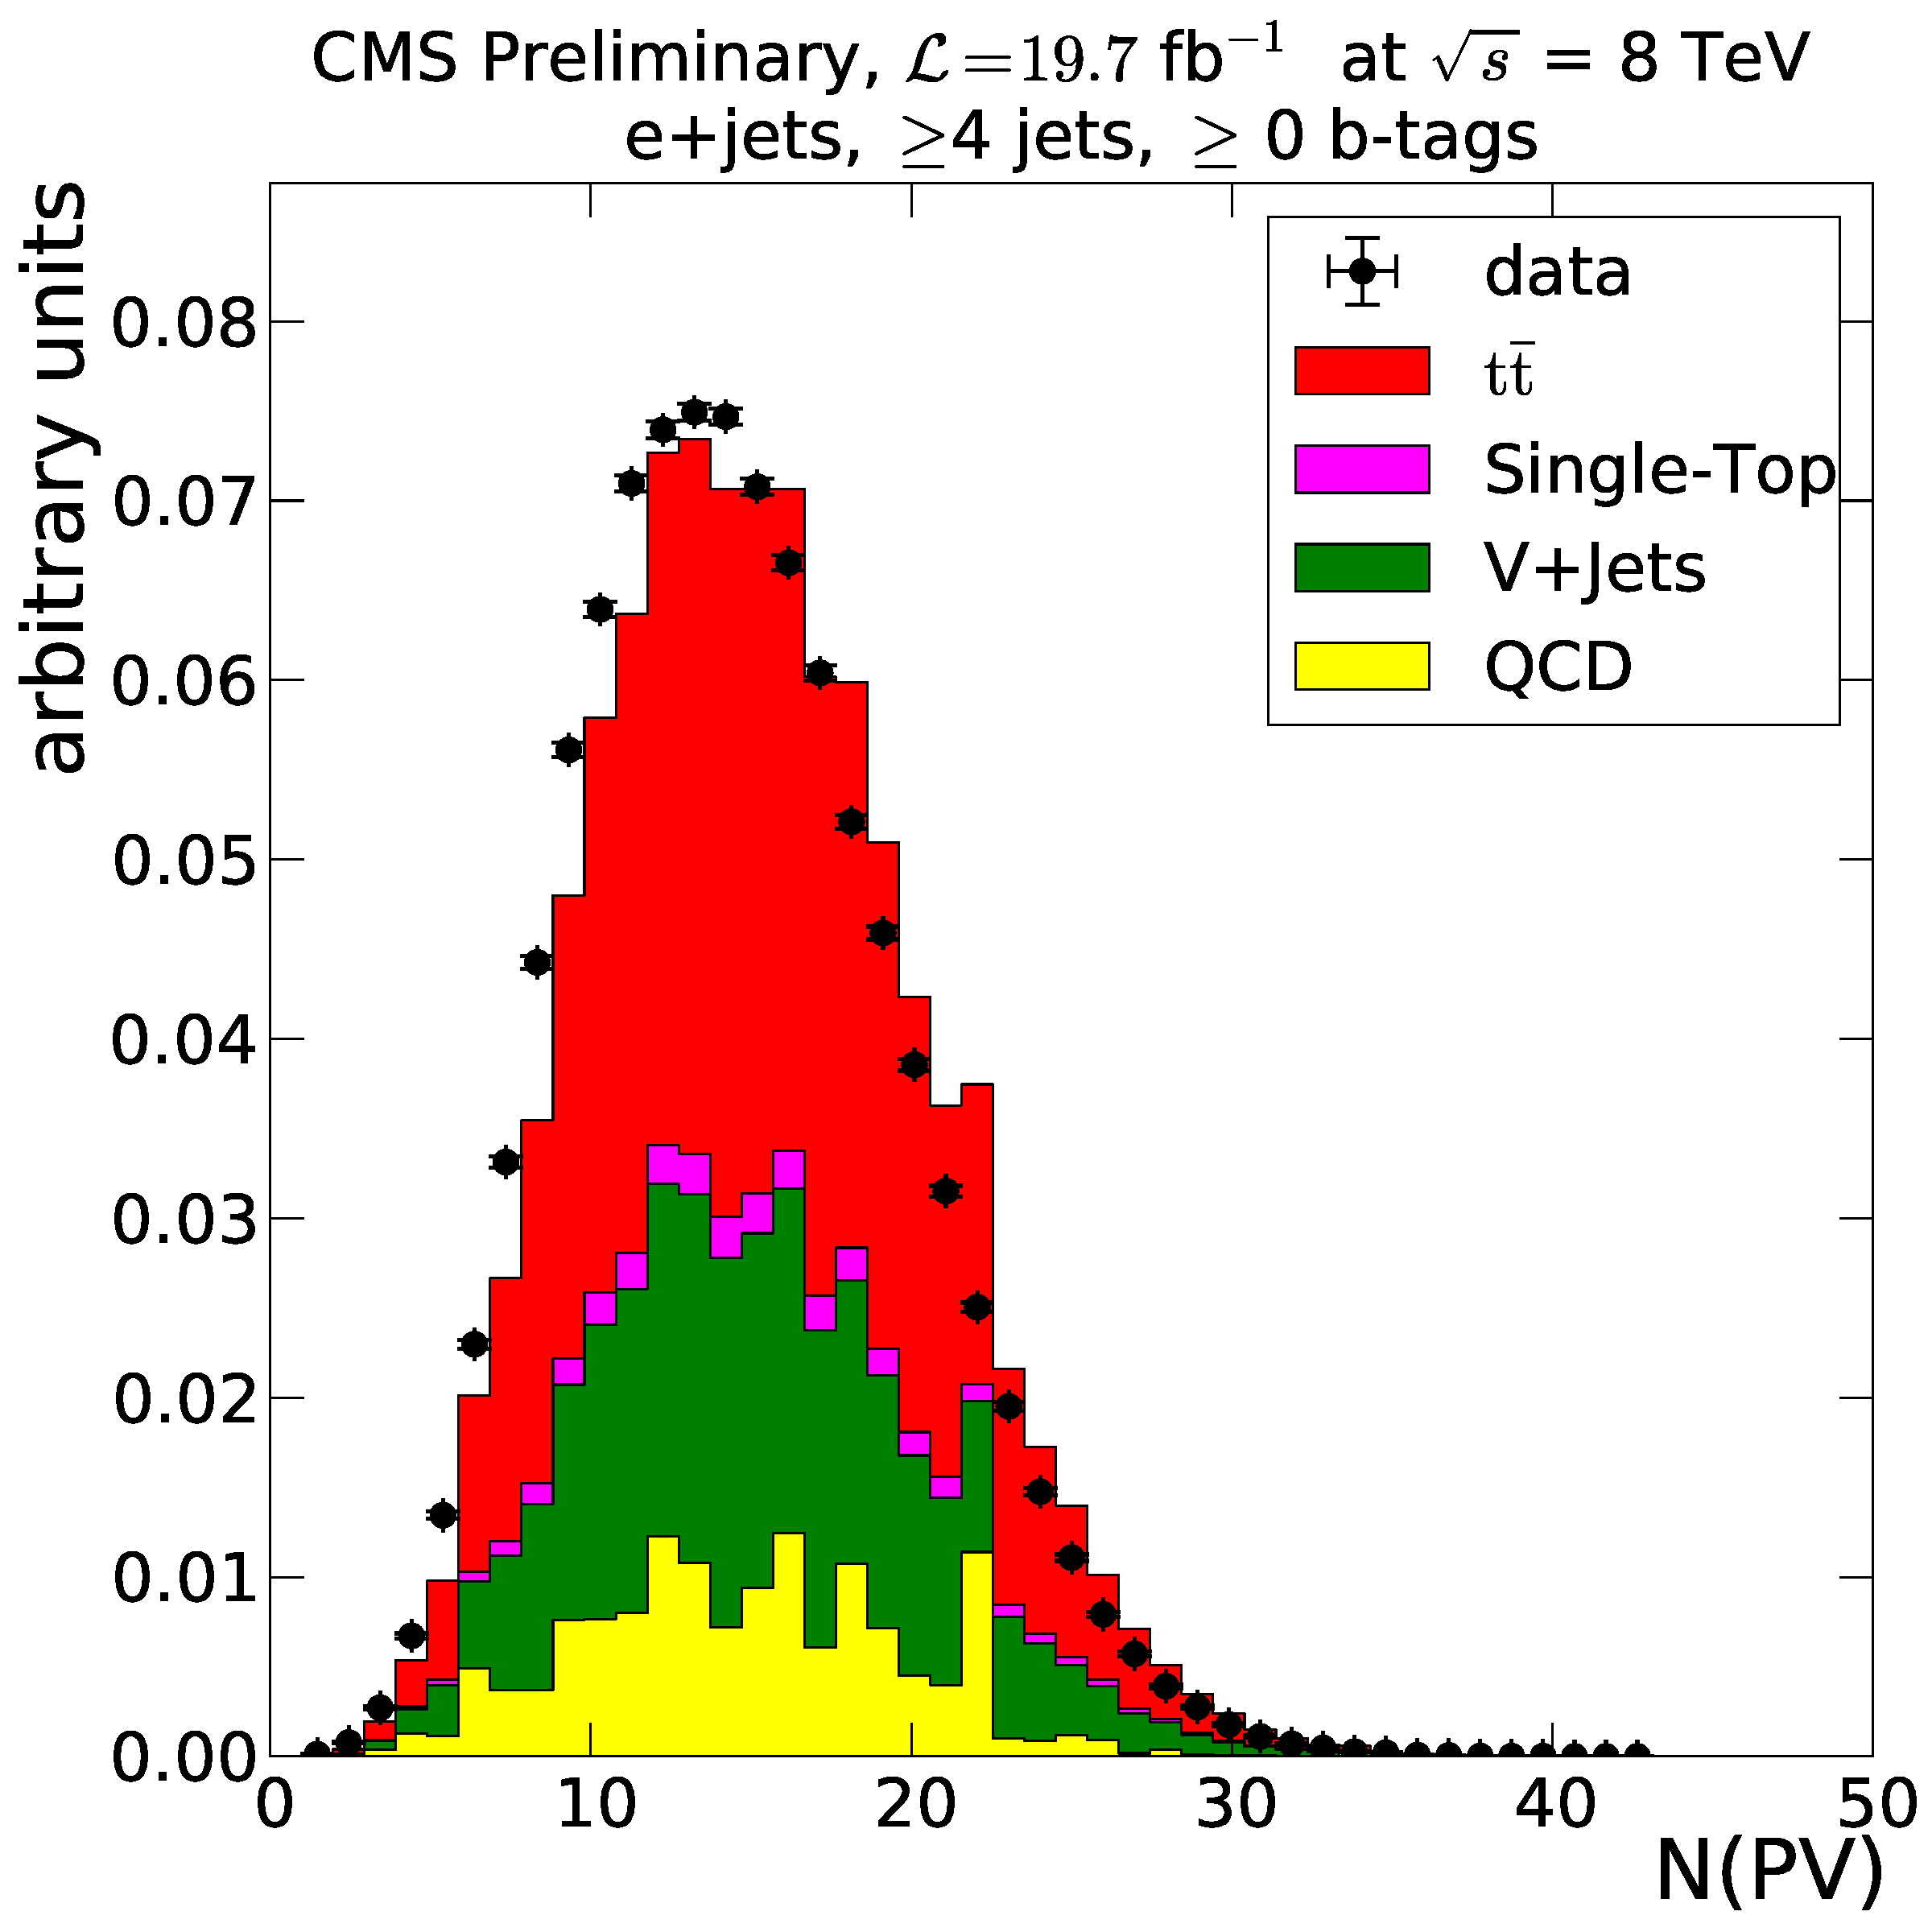
\includegraphics[width=0.50\textwidth]{vertices/EPlusJets_nVertex_reweighted_PU_up.pdf}} \\
	\subfloat[]{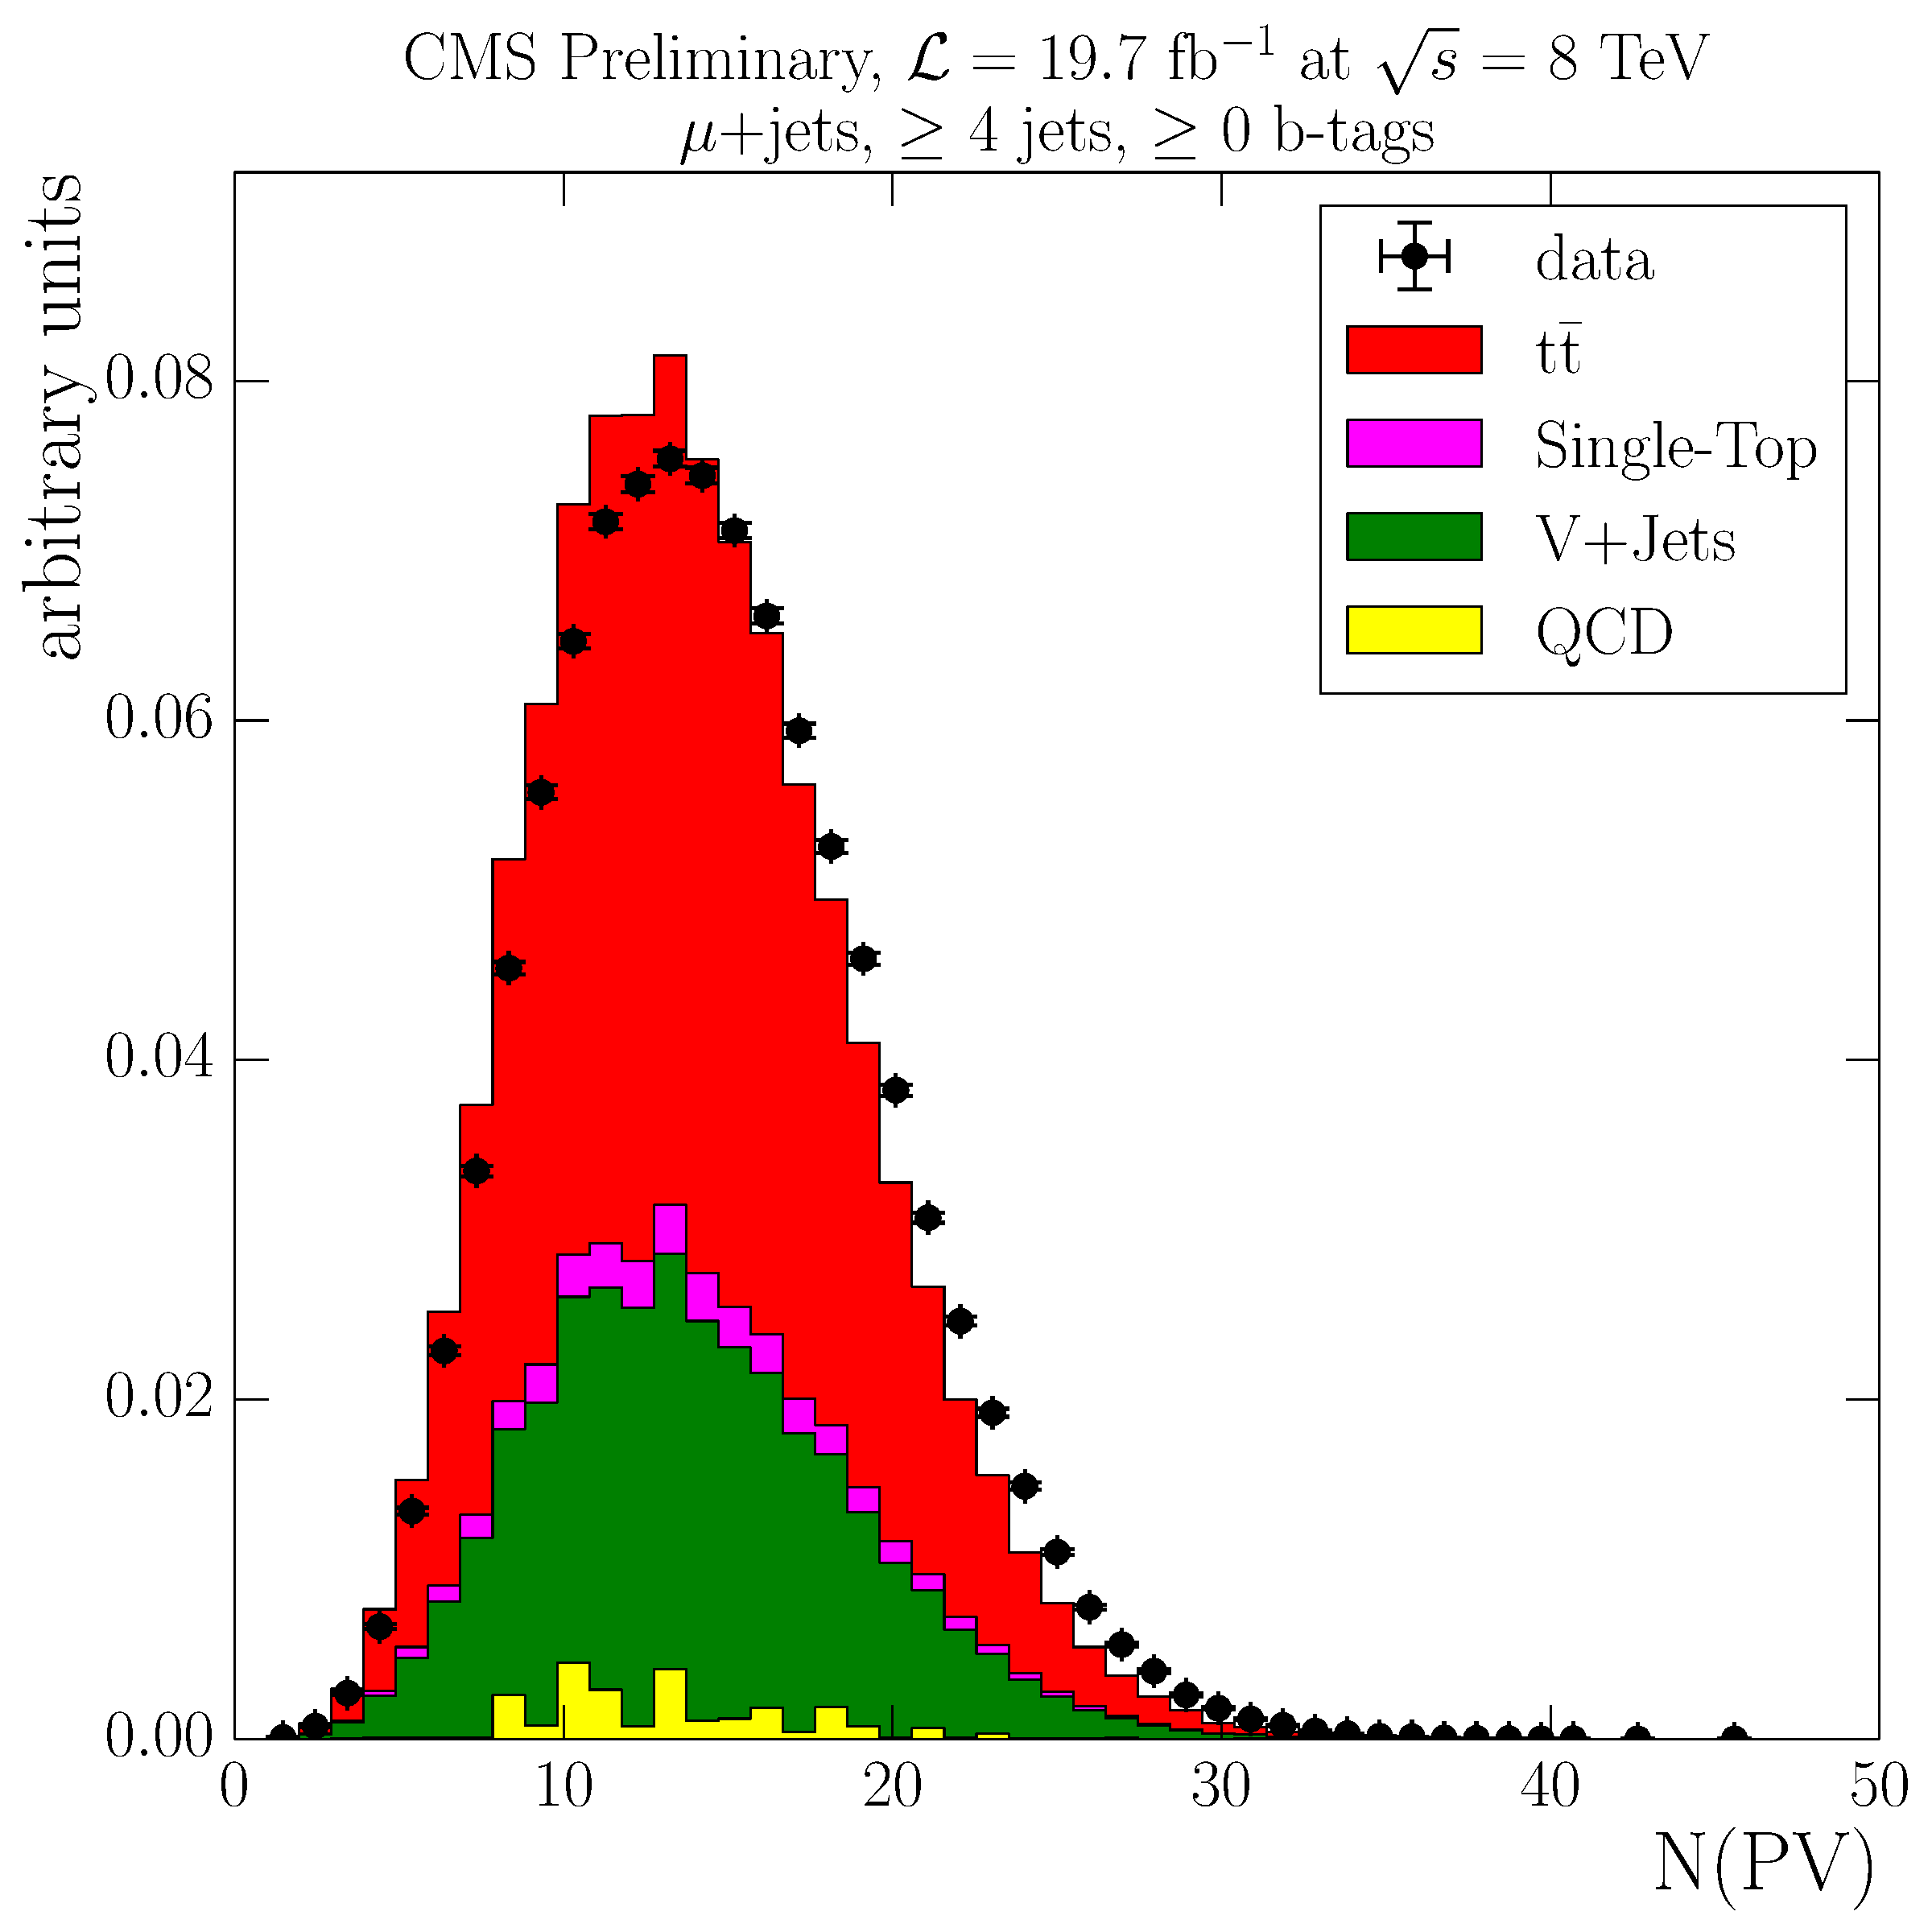
\includegraphics[width=0.50\textwidth]{vertices/MuPlusJets_nVertex_reweighted_PU_down.pdf}}\hfill
	\subfloat[]{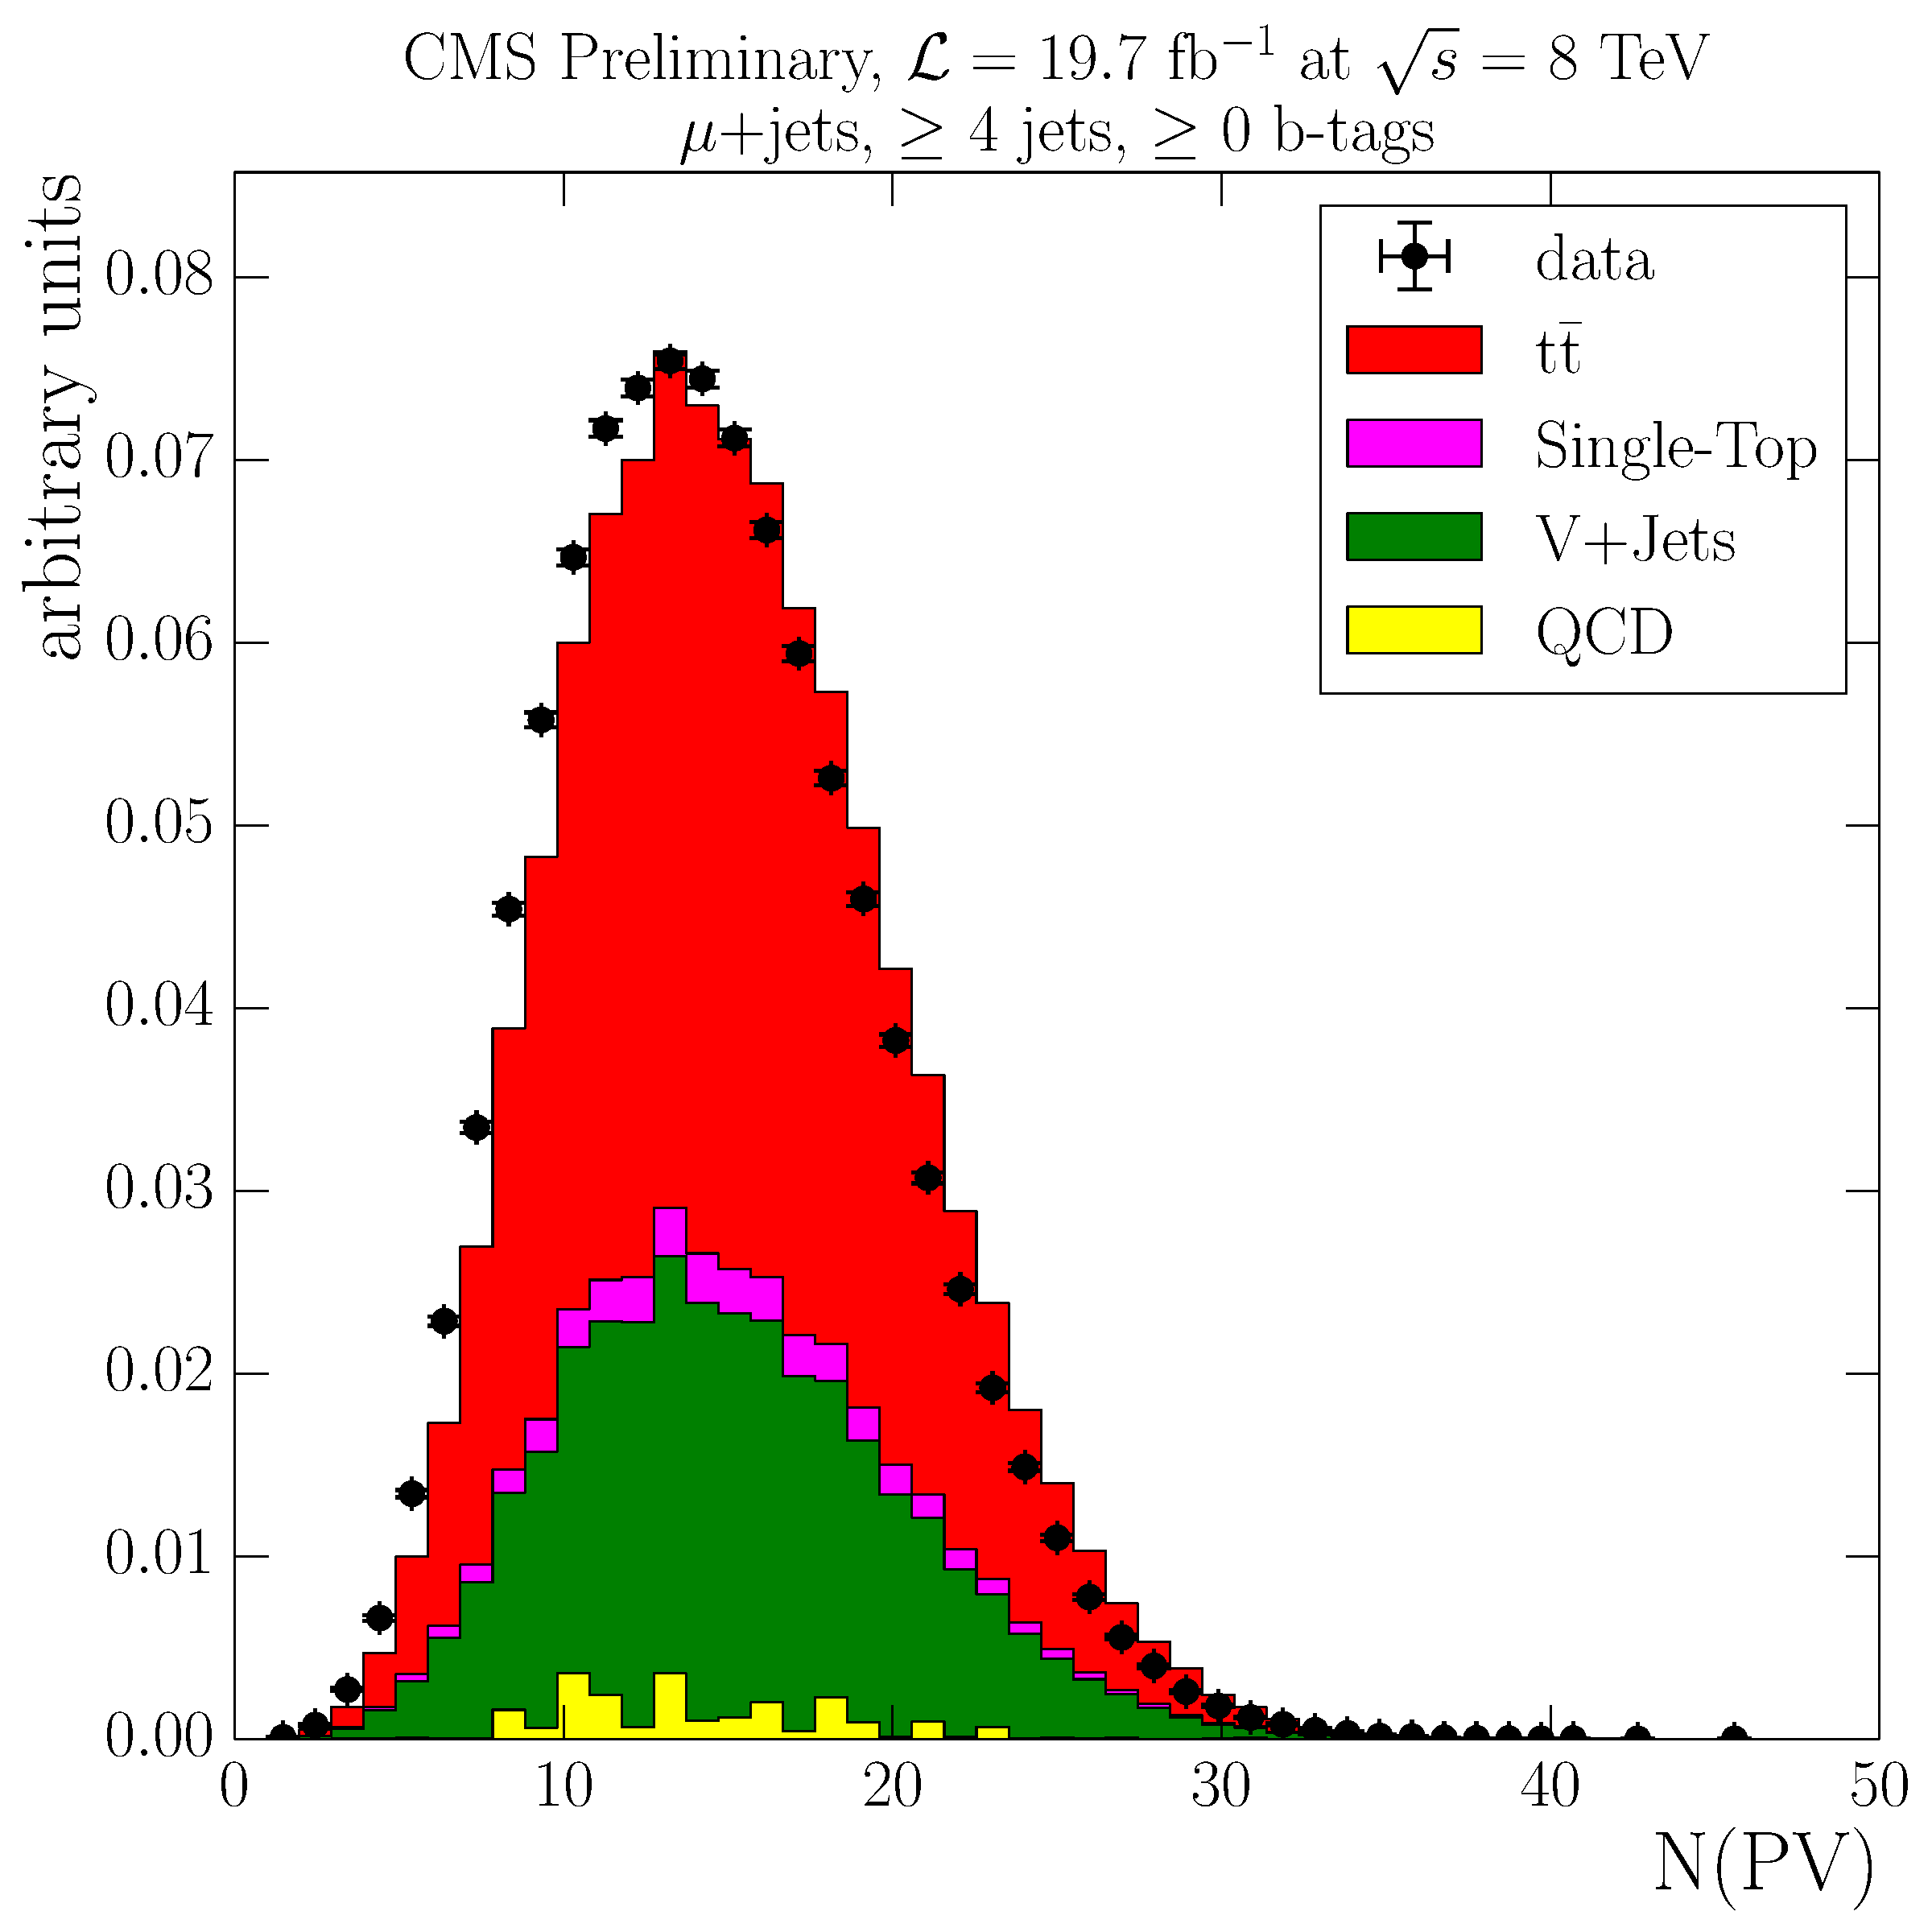
\includegraphics[width=0.50\textwidth]{vertices/MuPlusJets_nVertex_reweighted_PU_up.pdf}}
	\caption{\label{fig:pileup_vertices_variations}
    Number of reconstructed vertices per event for the $-\sigma$ (left) and the $+\sigma$ variations (right) of
    the pile-up reweighting procedure for the electron channel (top) and the muon channel (bottom).}
\end{center}
\end{figure}


\subsection{b-tagging corrections}
\label{ss_xsection:btagging_corrections}
%EDIT
% In this analysis $b$ tagging is used in the event reconstruction to associate reconstructed jets to partons in the decay
% chain and to select events in the final analysis. Here, the \emph{combined secondary vertex} tagger with the medium
% operation point  (cut value~0.679, CSVM) is used which results in a $1\%$ light-jet mistag rate ~\cite{CMSbAlgo}.

% We apply \pt dependent b-tag efficiency corrections to each $b$ tag for simulated events to account for the differences
% between data and simulation seen in 2012 data~\cite{bTagResultsPaper}. Simulated events passing the $b$ tagging
% requirements are given a weight (following the prescription from the BTag POG~\cite{bTagWeight}) to ensure that the
% probability of selecting a simulated event matches the probability of a data event with the same jet flavour composition
% being selected.

% The results of the reweighting can be seen in fig. \ref{fig:bjet_weights}. The number of MC events in the 0 and 1 b-tag
% is scaled up while the number of MC events with b-tag multiplicity higher than 2 are scaled down.


\begin{figure}[!htpb]
\begin{center}
	\subfloat[]{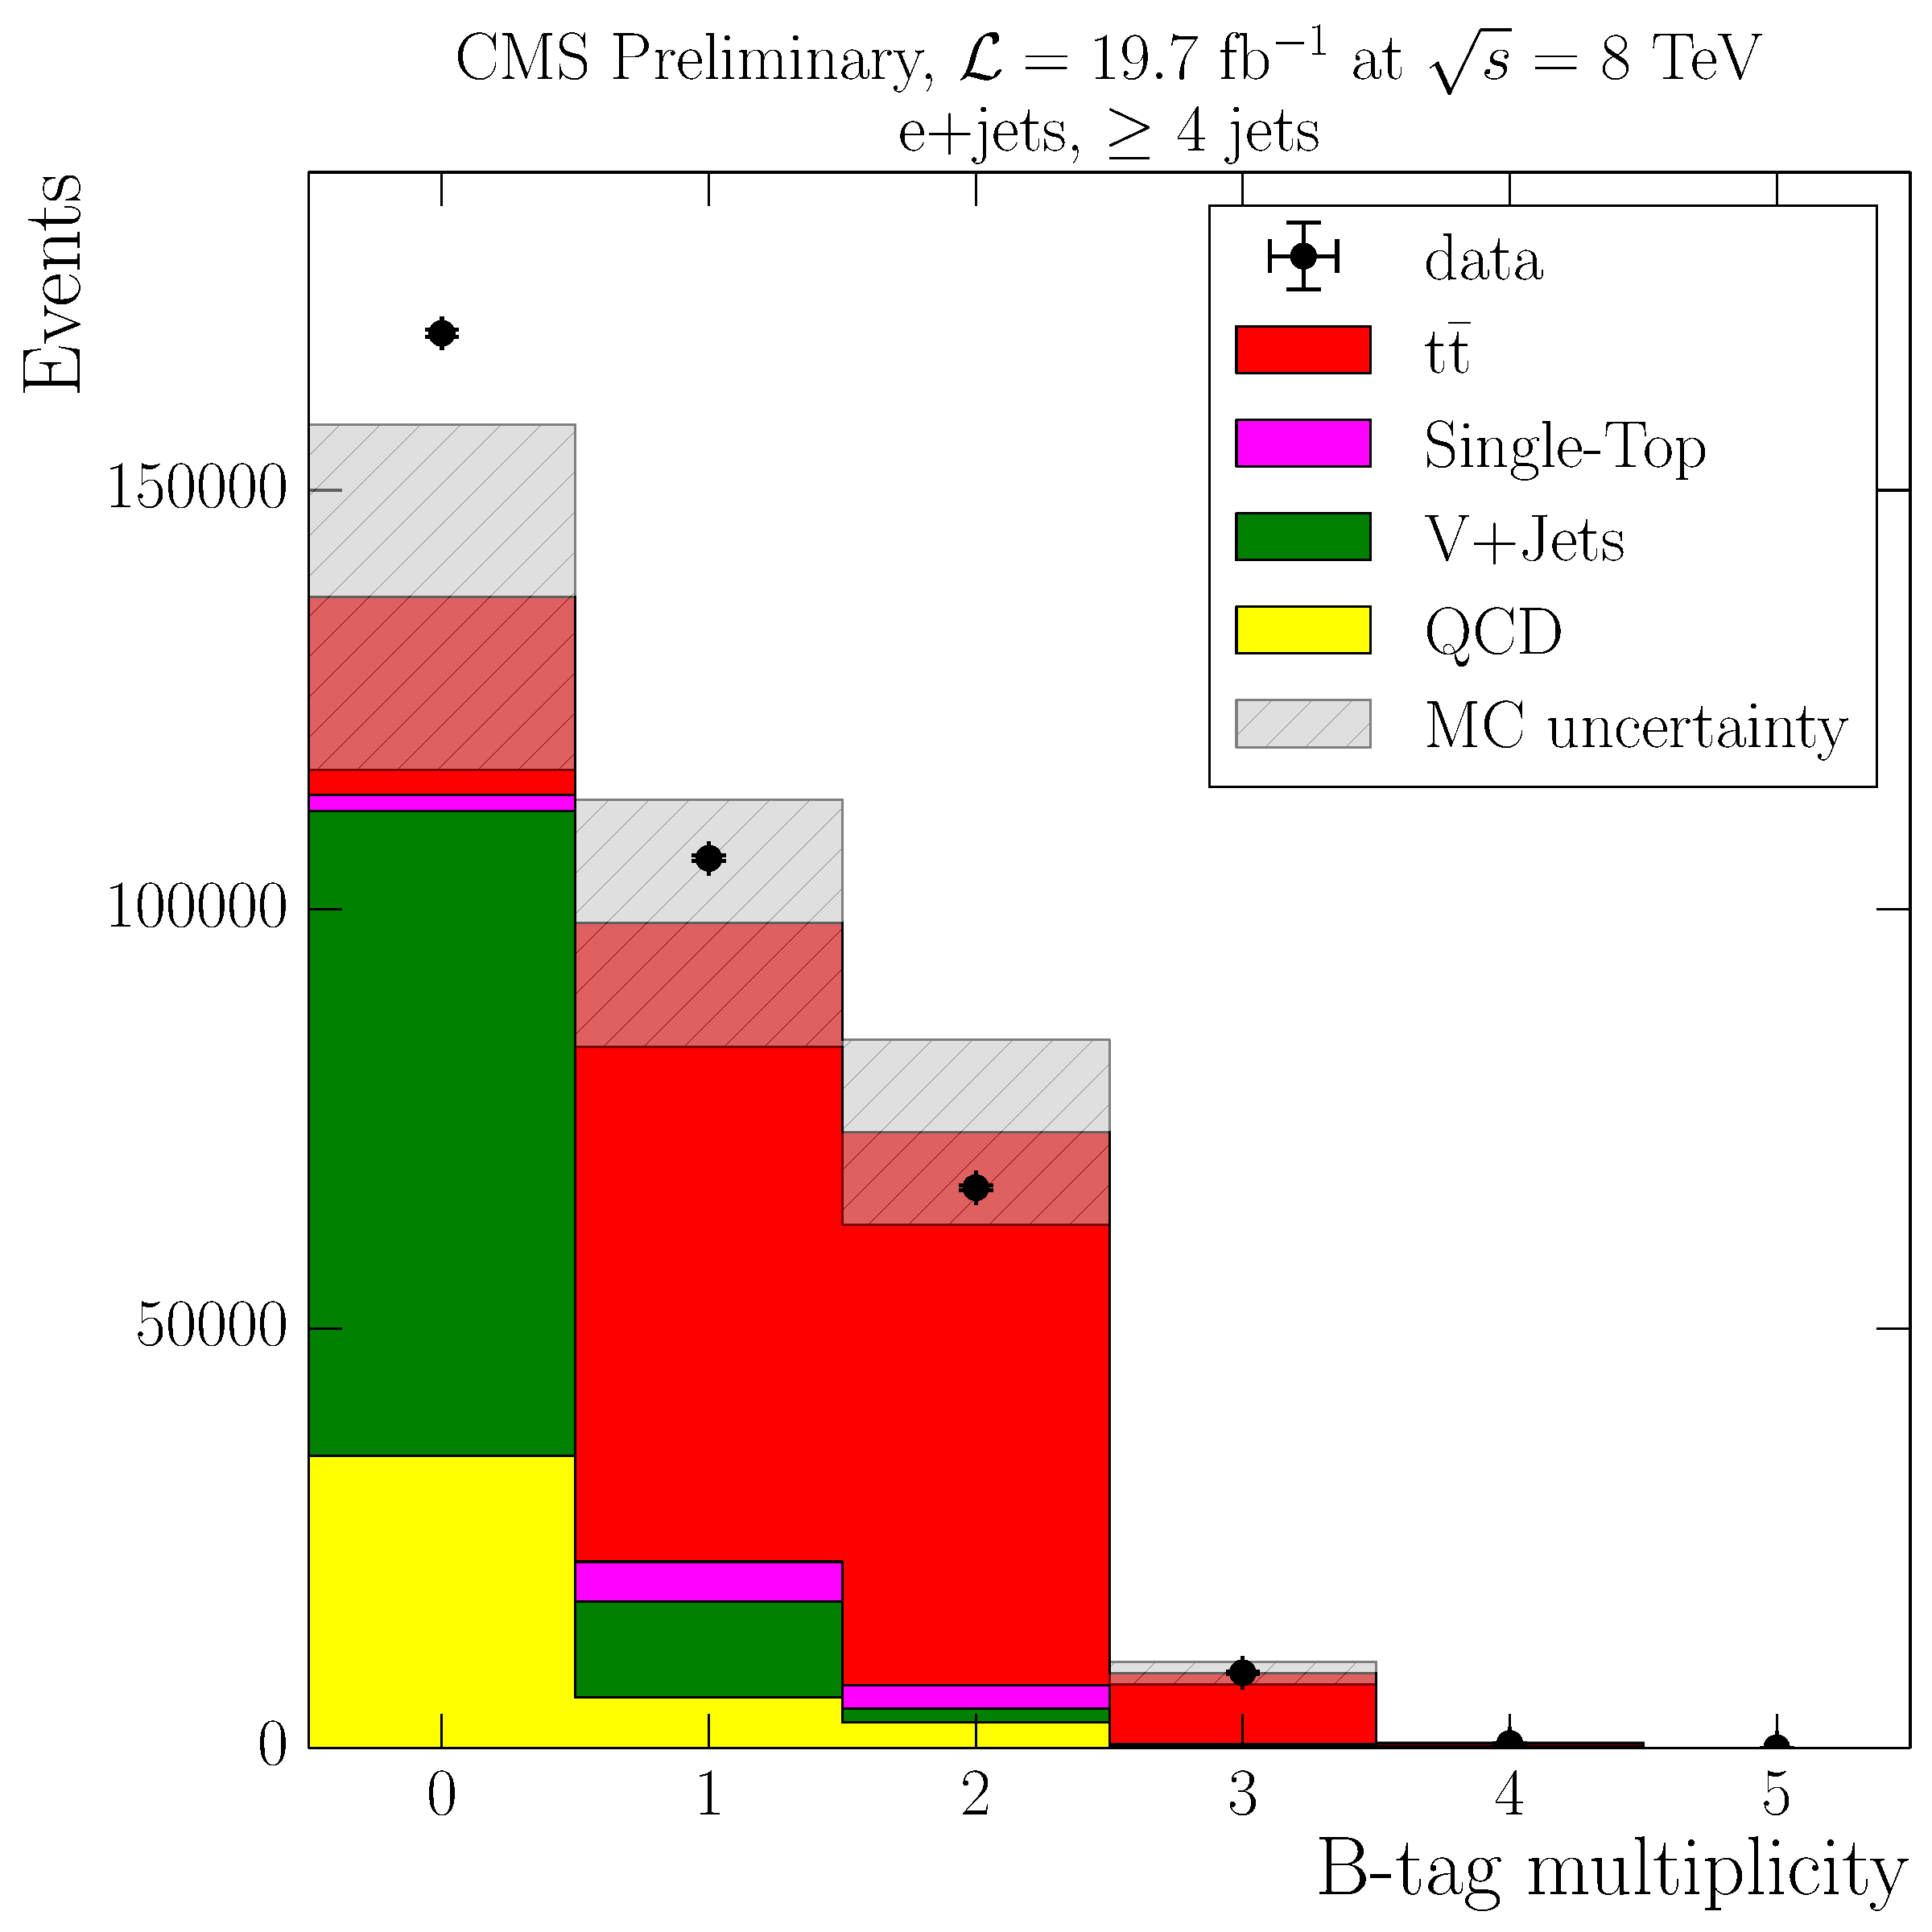
\includegraphics[width=0.50\textwidth]{bjets_multiplicity/EPlusJets_N_BJets.pdf}}\hfill
	\subfloat[]{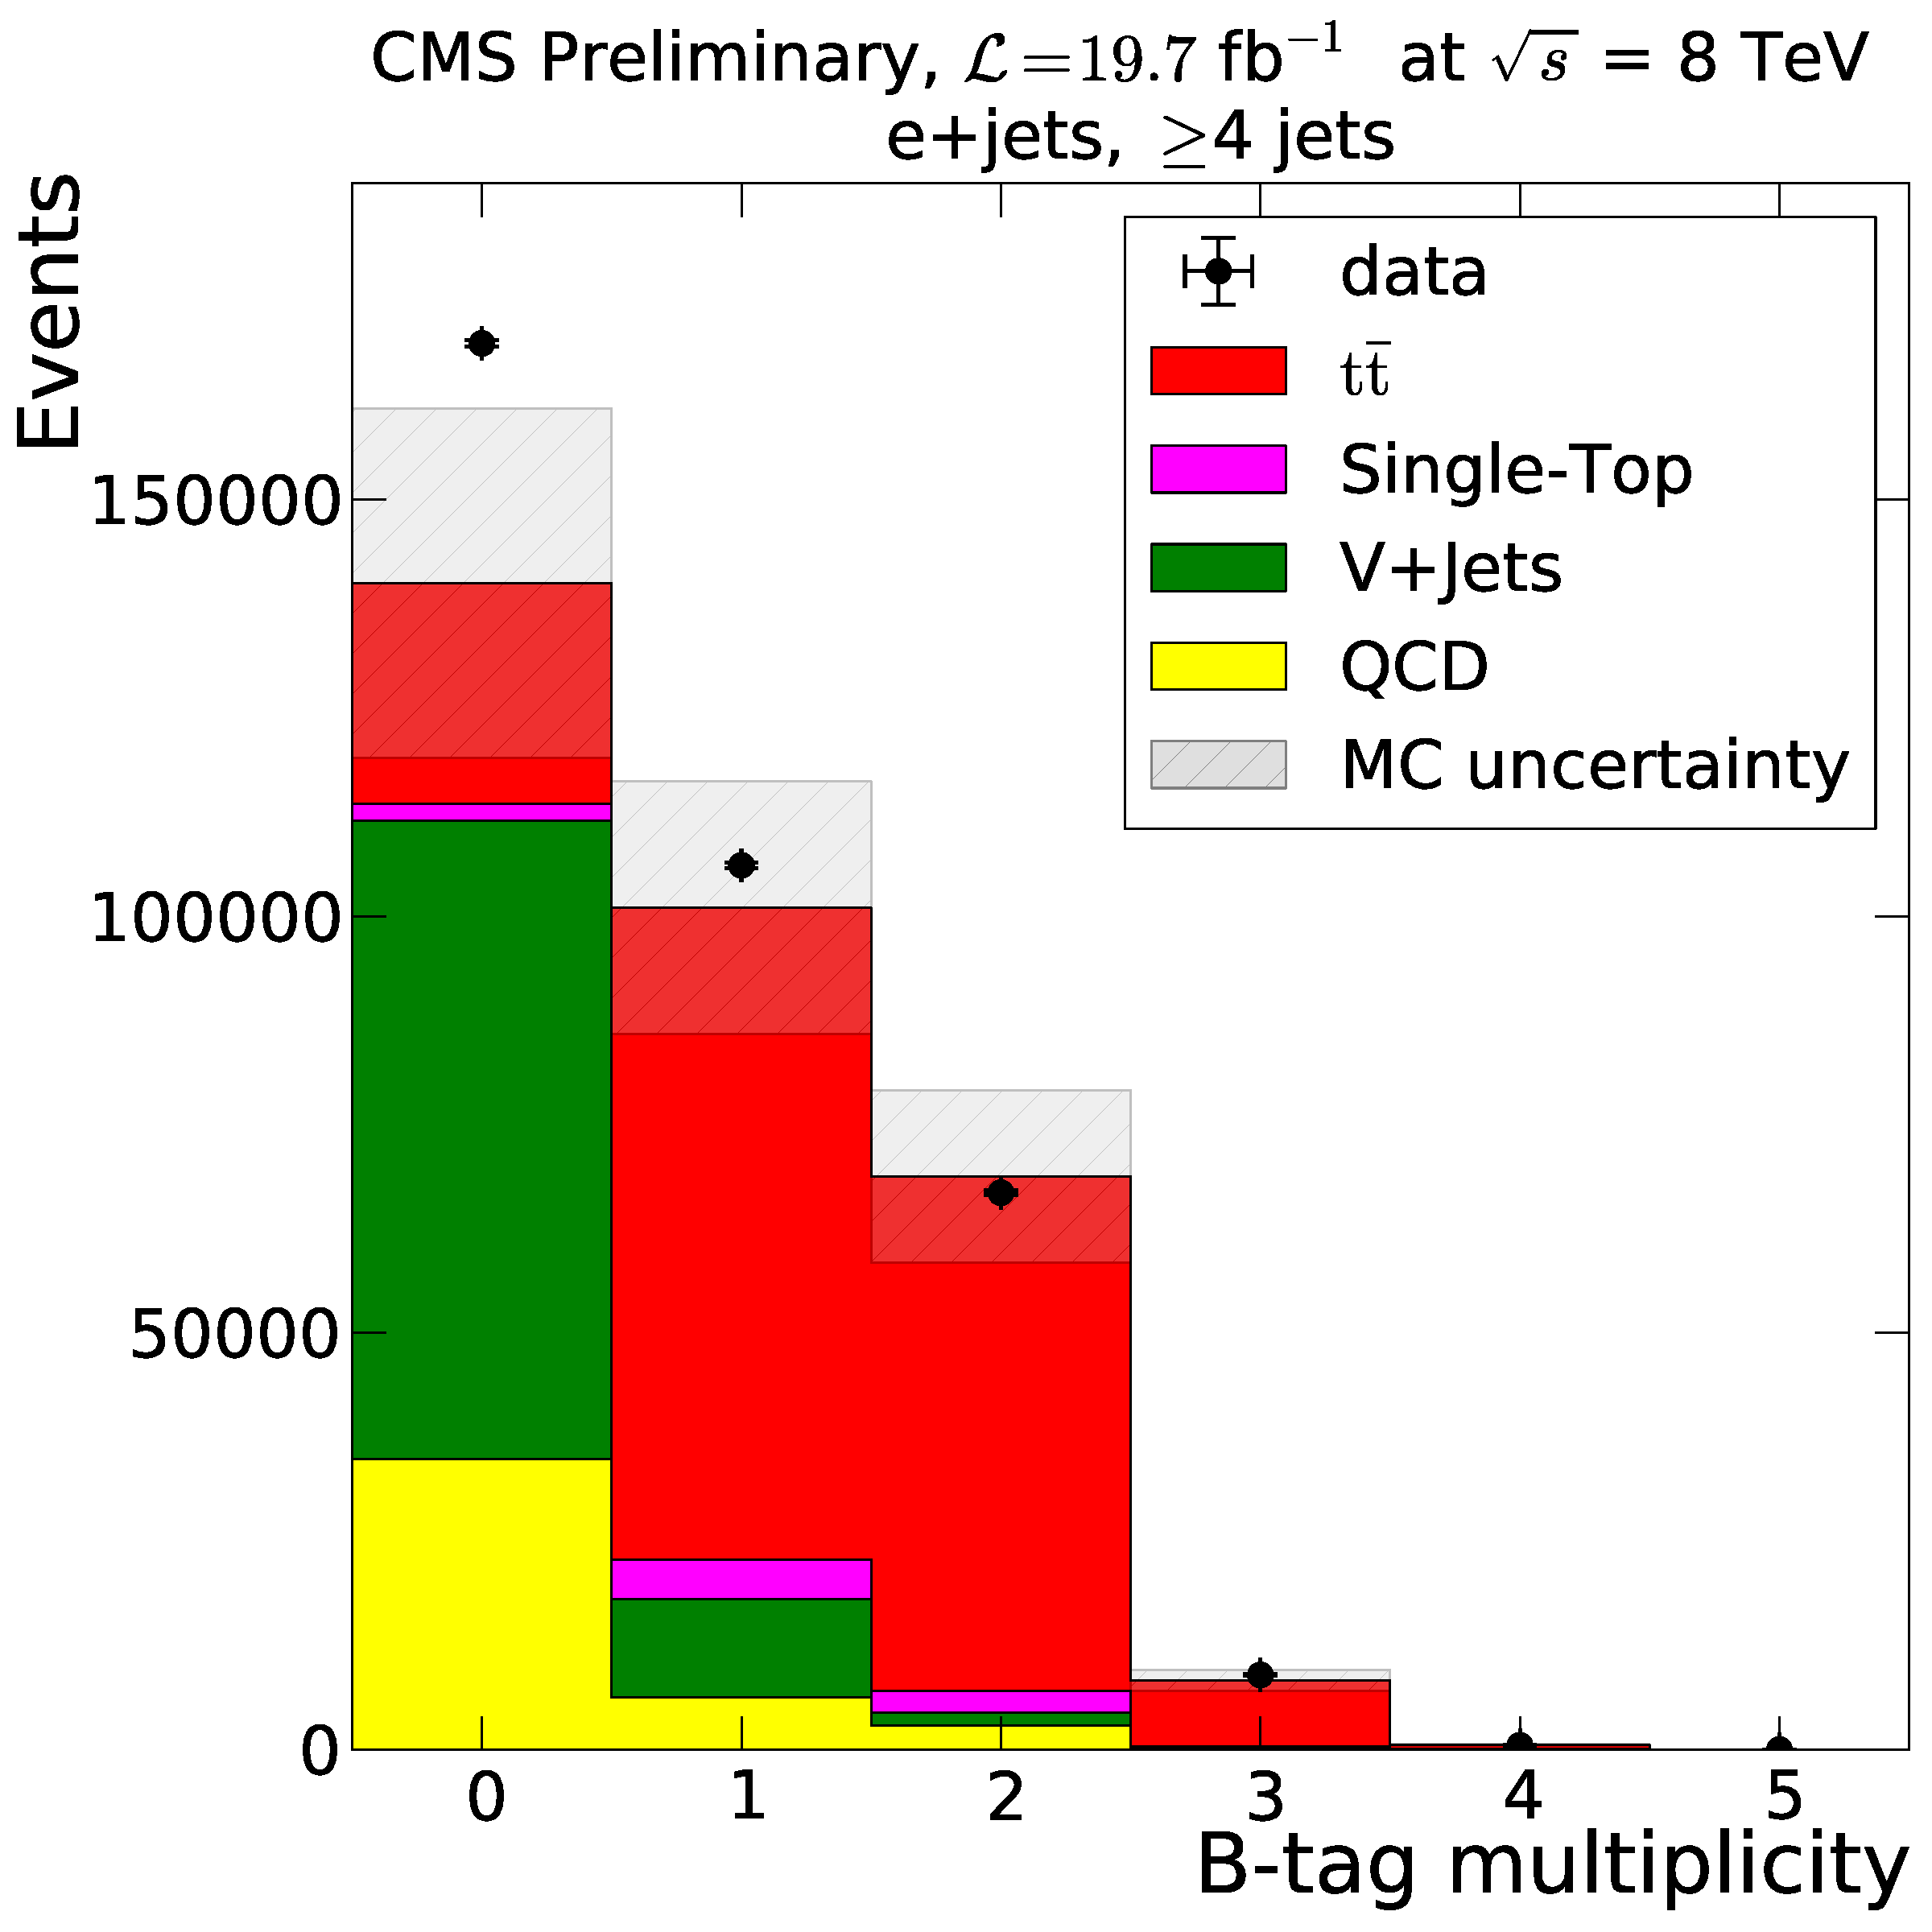
\includegraphics[width=0.50\textwidth]{bjets_multiplicity/EPlusJets_N_BJets_reweighted.pdf}} \\
	\subfloat[]{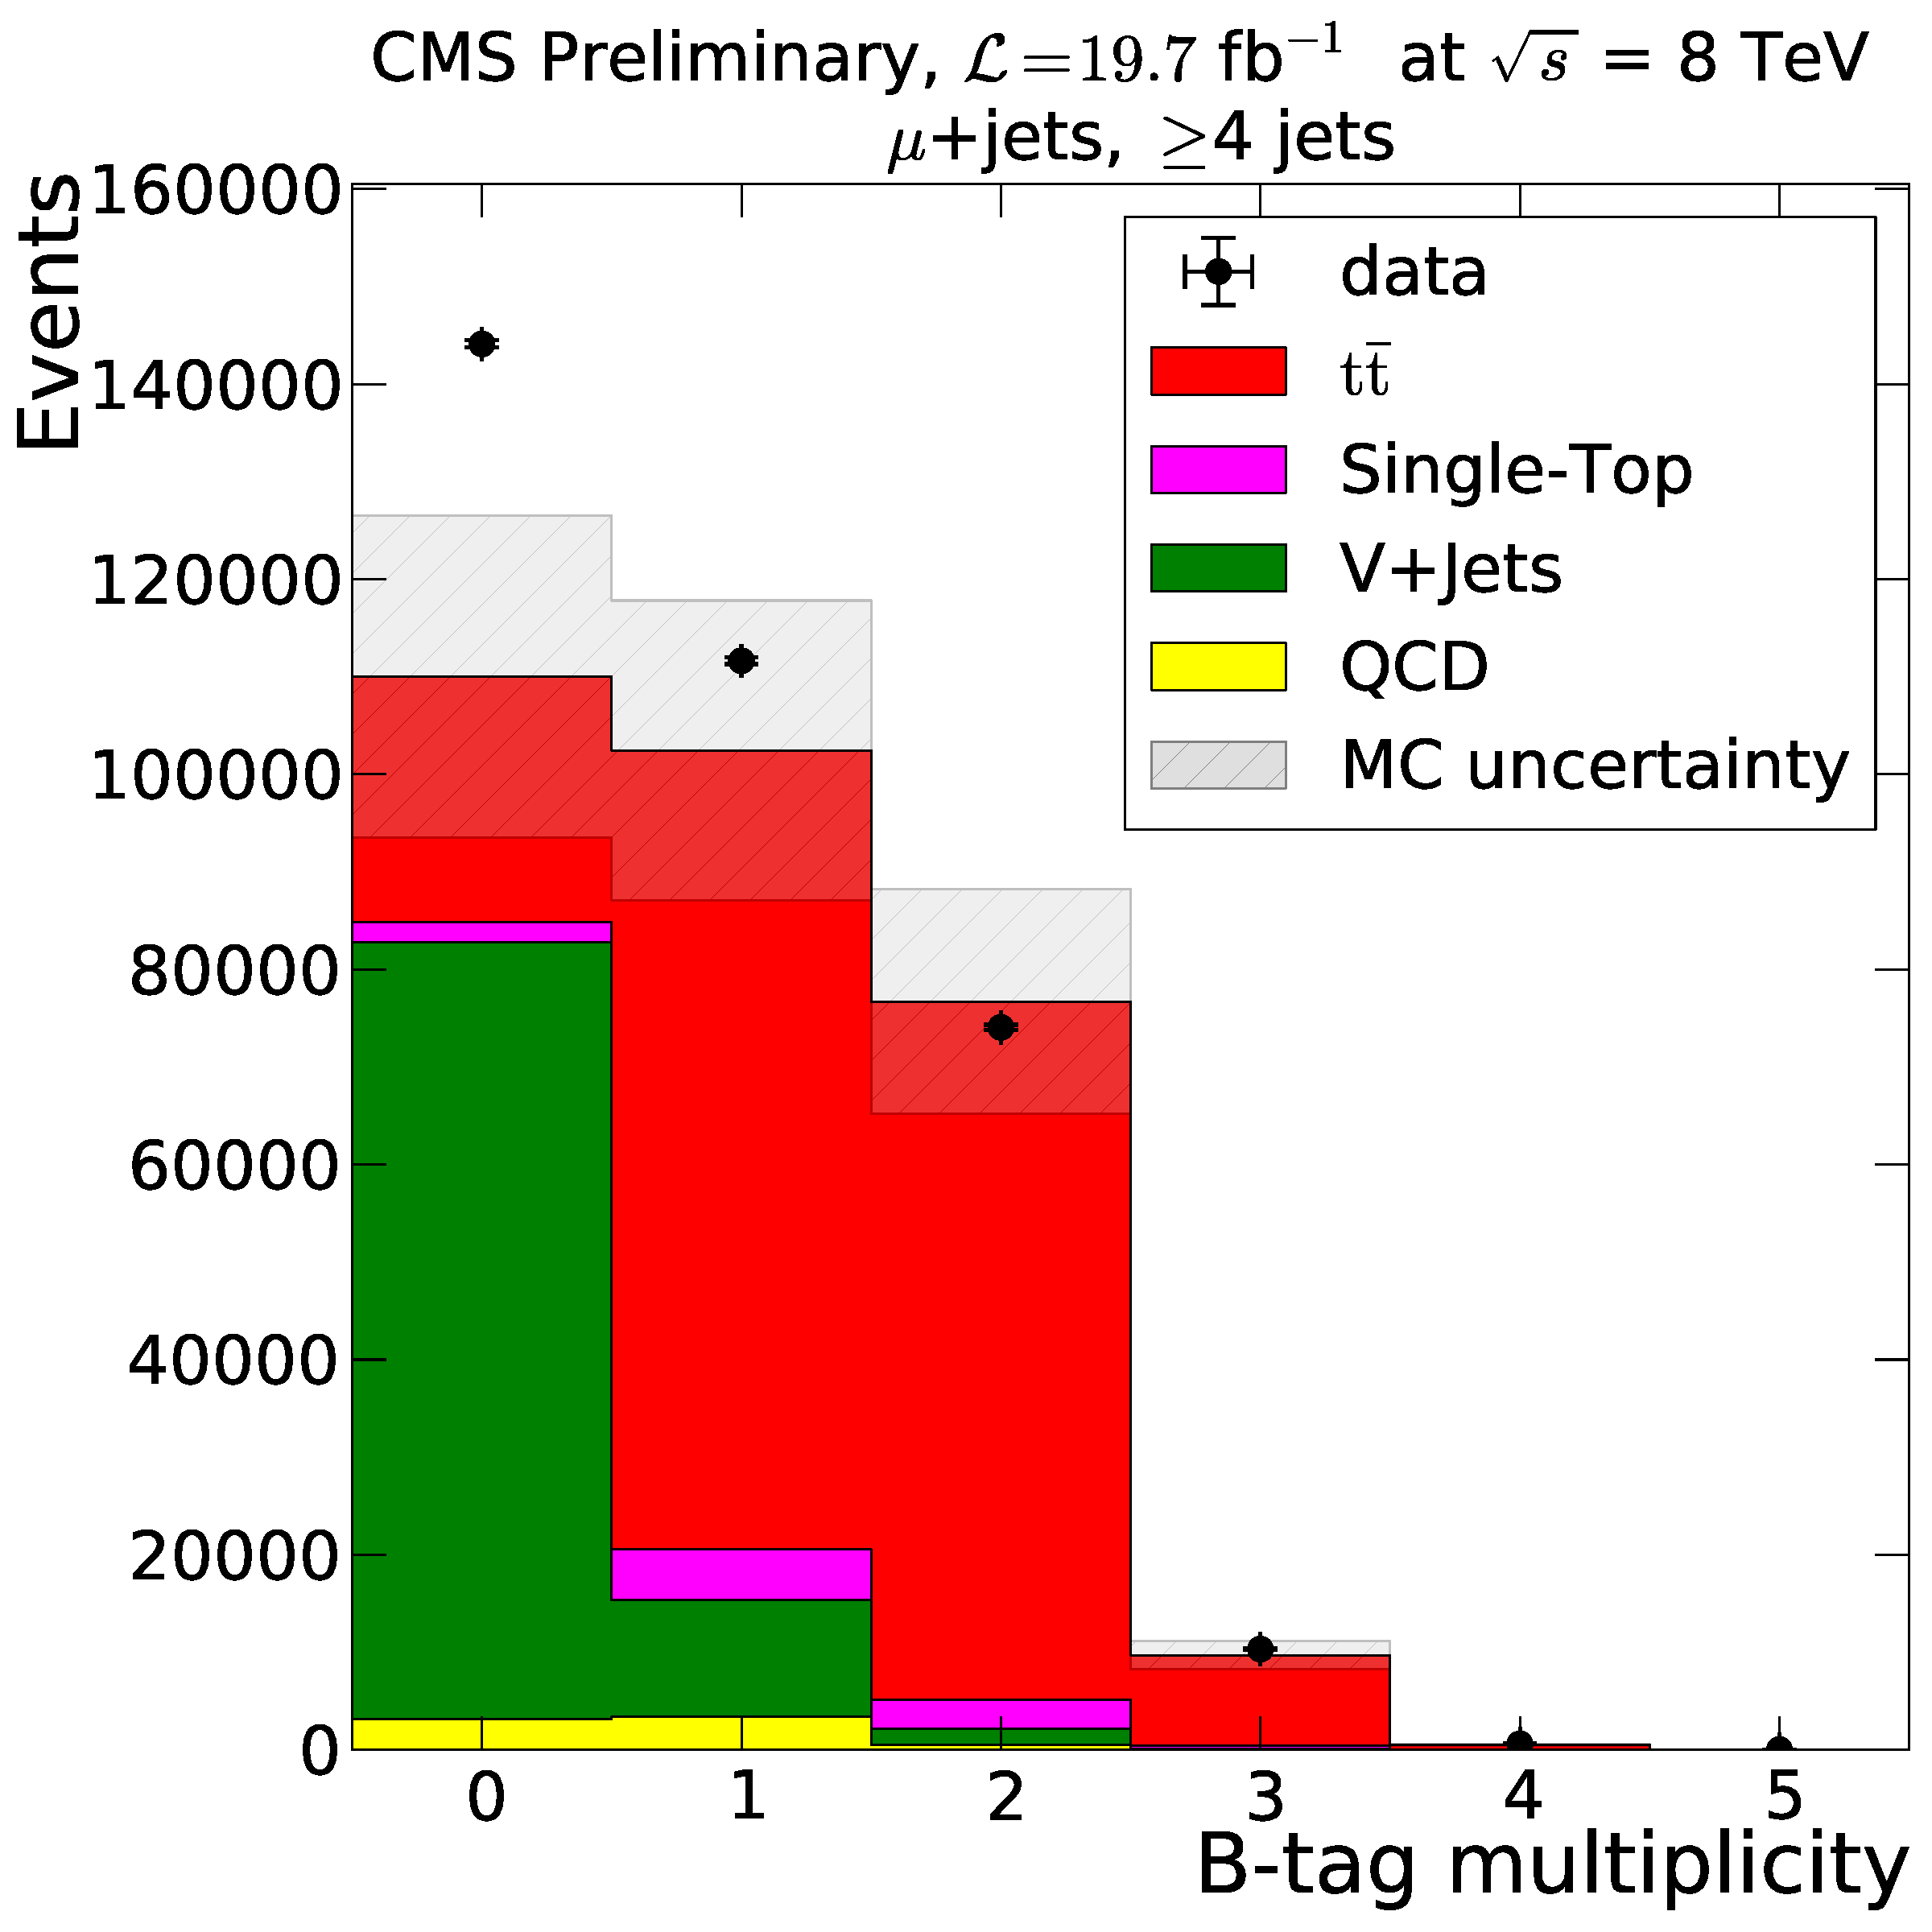
\includegraphics[width=0.50\textwidth]{bjets_multiplicity/MuPlusJets_N_BJets.pdf}}\hfill
	\subfloat[]{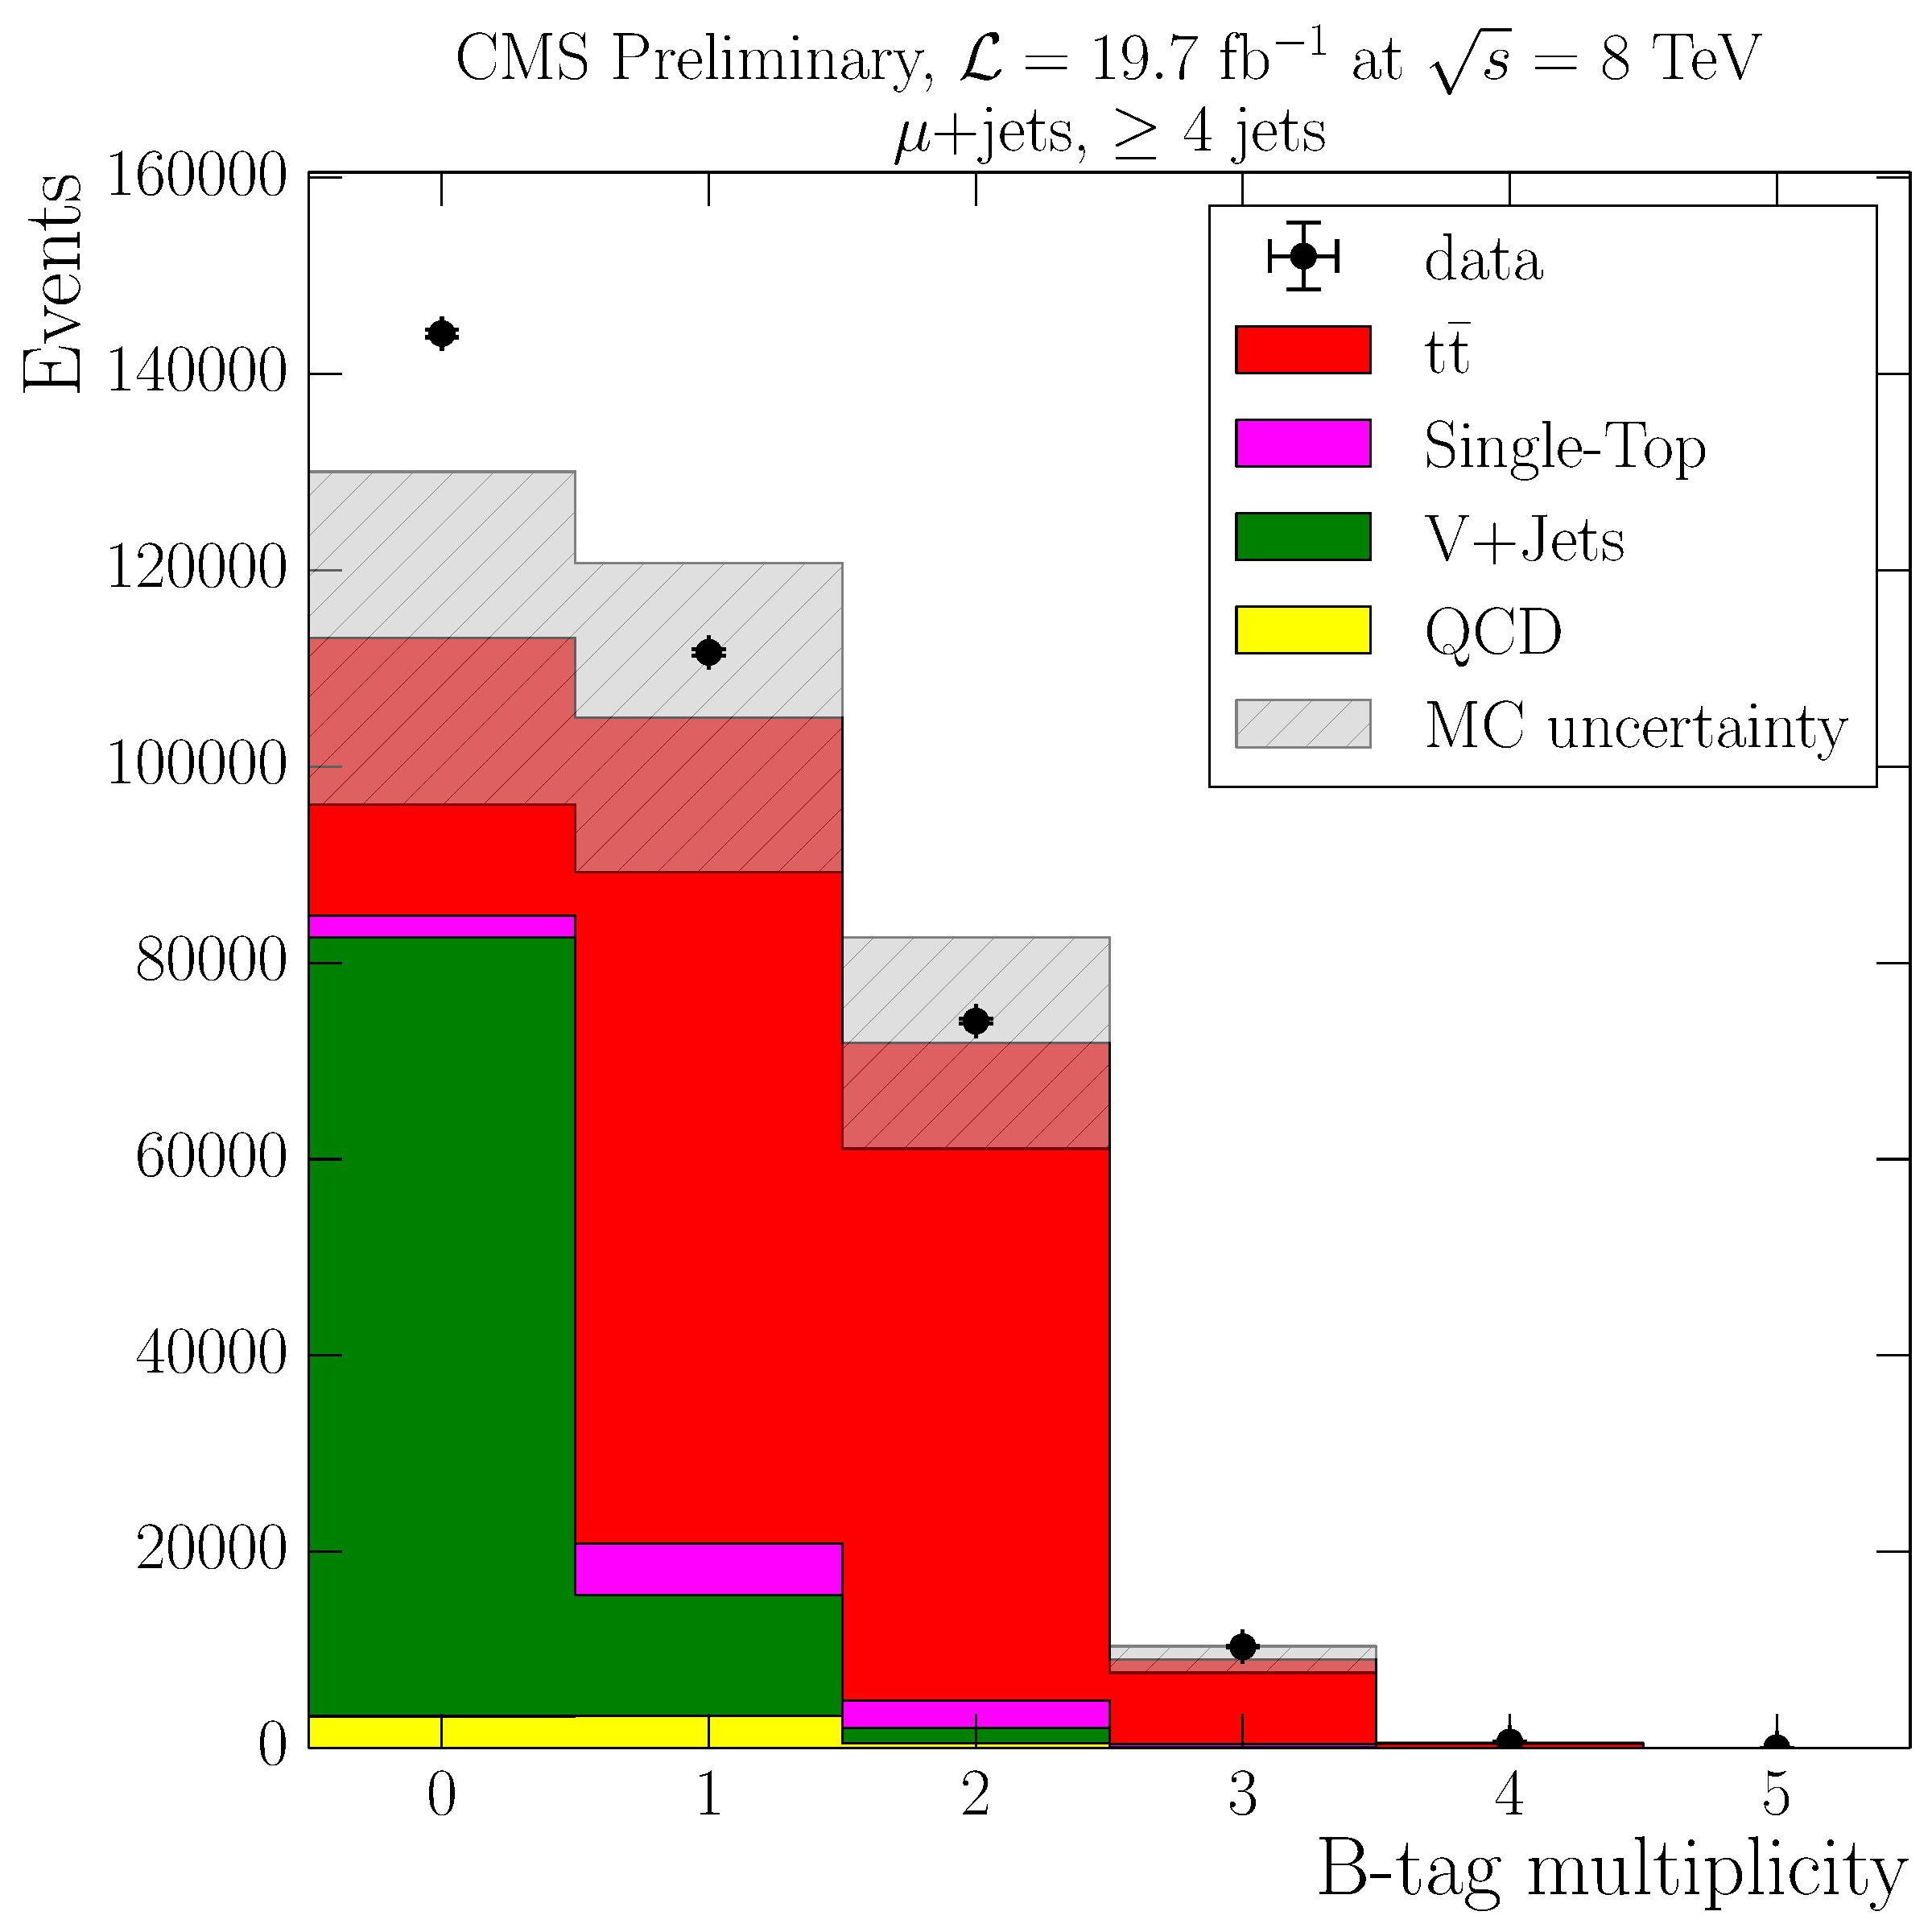
\includegraphics[width=0.50\textwidth]{bjets_multiplicity/MuPlusJets_N_BJets_reweighted.pdf}}
	\caption{\label{fig:bjet_weights}
    b-tag multiplicity before (left) and after applying b-tag scale factors (right) in the electron channel (top) and
    the muon channel (bottom).}
\end{center}
\end{figure}

% The systematic variations of the uncertainties due to the $b$ tag efficiency are applied by varying the efficiency scale
% factor $SF$ by the according $\pm 1 \sigma$ variations in the event reweighting procedure.

\section{Event Selection}
\label{s_xsection:event_selection}
As in the top quark mass analysis, the event selection in this work is based on the standard CMS selection optimised for
the Standard Model \ttbar production. It also exploits the semi-leptonic signature of a \ttbar decay with exactly one
isolated lepton and at least four jets, two of which are b-tagged. One of the main goals of the analysis is the
measurement of the missing transverse energy distribution represented by a neutrino from the leptonic decay of the \W
boson, however, there is no specific requirement on the \MET in the selection.

Comparing to the 2011 event selection described in Section~\ref{s_top_mass:event_selection}, enhanced pile-up
subtraction and lepton identification techniques are used. Improved understanding of the detector in form of updated
alignment and calibration constants resulted in better resolution of jets and \MET. The preselection (or skimming) step
used in order to reduce the number of events for local analysis processing is identical to that of 2011 analysis.
However, additional filters are used to reject the events with artificial \MET caused by noise or known problems with
one of the detector subsystems. These filters are discussed in Section~\ref{ss_xsection:met_filters}.

Two semi-leptonic \ttbar decay modes are explored in this analysis: the electron plus jets and the muon plus jets
channels. The event selection for each of these decay modes is described below.

\subsection{Electron plus jets channel}
\label{ss_xsection:ejets}

Similarly to the electron plus jets channel in the top quark mass analysis, the selection consists of the following
steps:

\begin{enumerate}[topsep=\parskip, parsep=\parskip, itemsep=\parskip, leftmargin=\leftmargin]
	\item preselection;
	\item trigger;
	\item electron candidate selection;
	\item dilepton veto;
	\item conversion veto;
	\item muon veto;
	\item jet selection;
	\item b-tagging.
\end{enumerate}

%https://twiki.cern.ch/twiki/bin/view/CMS/TWikiTop2011DataMCTrig

\subsubsection*{Trigger}
As opposed to 2011 analysis using cross triggers, a single electron trigger is used in this analysis. Referred to as
HLT\_Ele27\_WP80, this trigger has a lepton \pt threshold of \SI{27}{\GeV} and ``WP80'' lepton isolation requirement
(see Table~\ref{tab:trigger_naming}), but no specific jet requirements. In contrast to 2011 data-taking, the single
electron trigger was unprescaled for the whole period of 2012 running, despite a comparatively large rate. This decision
was made due to simplicity of the trigger selection, requiring flat efficiency corrections.

\subsubsection*{Electron candidate selection}
Similarly to 2011 selection, exactly one electron candidate passing is required in the event, passing the following
criteria:

\begin{itemize}
	\item $\ET > \SI{30}{\GeV}$;
	\item $|\eta| < 2.5$, excluding the ECAL barrel-endcap transition regions of $1.4442 < |\eta| < 1.566$;
	\item MVA electron ID (Section~\ref{ss:electron_reconstruction}) with a discriminator cut of $>0.5$;
	\item transverse impact parameter with respect to the primary vertex $d_{xy} < \SI{0.02}{\cm}$;
	\item PF-based relative isolation (Section~\ref{sss:electron_isolation}) \reliso $< 0.1$ with a $\Delta
R$ cone of \num{0.3}.
\end{itemize}

\subsubsection*{Dilepton veto}
To reject events with additional electrons, dilepton veto is applied. Events are rejected if they contain a second
electron candidate with the same ID and $\eta$ requirements, but looser \ET and \reliso criteria ($>\SI{20}{\GeV}$ and
$<0.15$, respectively).

\subsubsection*{Conversion veto}
As described in Section~\ref{sss:photon_conversions}, a vertex fit technique combined with the number of missing hits
in the tracker is used for photon conversion rejection.

\subsubsection*{Muon veto}
To reduce contamination from other \ttbar decay modes (i.e.\ muon and dilepton channels), events containing a global or
a tracker muon (see Section \ref{ss:muon_reconstruction}) are rejected. The requirements on the muon are identical to
those of 2011 selection: $\pt > \SI{10}{\GeV}$, $|\eta| < 2.5$ and $\reliso < 0.2$ with a $\Delta R$ cone of \num{0.4}.

\subsubsection*{Jet selection and b-tagging}
To help further reduce the background, at least four jets with $\pt > \SI{30}{\GeV}$ and $|\eta| < 2.5$ are required in
the event. These jets are required to pass the loose PF jet ID (see Section \ref{ss:jet_reconstruction}). Before the
multiplicity and identification requirements, the collection of jets is cleaned against the signal electron, i.e.\ any
jet within a $\Delta R$ cone of \num{0.3} around the signal lepton is excluded from the analysis. This is done due to
the fact that an electron may be reconstructed as a jet by leaving a characteristic signature in calorimeters. Any
additional jets with $\pt > \SI{20}{\GeV}$ and the same cleaning and ID requirements are also used for calculation of
\HT and \ST variables. Finally, the combined secondary vertex (CSV) b-tagging algorithm with the medium working point
(Section \ref{sss:b-tagging}) is used to identify the jets originating from \cPqb-quarks in the
\ttbar decay. At least two b-tagged jets are required in this analysis.

\subsection{Muon plus jets channel}
\label{ss_xsection:mujets}
The muon channel event selection follows similar strategy as that of the electron channel:

\begin{enumerate}[topsep=\parskip, parsep=\parskip, itemsep=\parskip, leftmargin=\leftmargin]
	\item preselection;
	\item trigger;
	\item muon candidate selection;
	\item second muon veto;
	\item electron veto;
	\item jet selection;
	\item b-tagging.
\end{enumerate}

\subsubsection*{Trigger}
An isolated single muon trigger, referred to as HLT\_IsoMu24\_eta2p1, is used in this channel. Partially suggested by
the name of the trigger path, the following criteria on the muon are imposed at the HLT level:

\begin{itemize}
	\item $\pt > \SI{24}{\GeV}$;
	\item $\abs \eta < 2.1$;
	\item Combined tracker and calorimeter-based relative isolation (Section~\ref{sss:electron_isolation}) \reliso $<
0.15$ with a $\Delta R$ cone of 0.3.

% according to https://twiki.cern.ch/twiki/bin/viewauth/CMS/MuonHLT isolation used to be 0.1, dR=0.24 in RunA
\end{itemize}

\subsubsection*{Muon candidate selection}
For selection of a muon candidate, exactly one muon satisfying the following requirements is required:

\begin{itemize}
	\item $\pt > \SI{26}{\GeV}$;
	\item $|\eta| < 2.1$;
	\item PF-based relative isolation (Section~\ref{sss:electron_isolation}) \reliso $< 0.12$ with a $\Delta
R$ cone of \num{0.4};
	\item PF-muon ID criteria (Section \ref{ss:muon_reconstruction}):
	\begin{itemize}
		\item identified as a particle flow muon and as a global muon;
		\item a normalised of the global muon fit $\chi^2<10$;
		\item number of muon chamber hits $>0$;
		\item number of muon stations with muon segments $>1$;
		\item transverse impact parameter w.r.t. the primary vertex $d_{xy} < \SI{0.02}{\cm}$;
		\item longitudinal distance of the tracker track w.r.t. the primary vertex $d_z < \SI{0.5}{\cm}$;
		\item number of hits in the pixel detector $>0$;
		\item number of hits in the tracker layers $>5$.
	\end{itemize}
\end{itemize}

\subsubsection*{Second muon veto}
Events containing an additional loose muon are rejected, with loose ID requirements as follows:

\begin{itemize}
	\item $\pt > \SI{10}{\GeV}$;
	\item $|\eta| < 2.5$;
	\item PF-based relative isolation (Section~\ref{sss:electron_isolation}) \reliso $< 0.2$ with a $\Delta
R$ cone of \num{0.4}; %PU corrections!
	\item identified as a particle flow muon, and either global or tracker muon.
\end{itemize}

These criteria are identical to the muon veto requirements in the electron channel.

\subsubsection*{Electron veto}
To further reduce background contamination, events with electrons are rejected. The requirements on additional loose
electron are the same to the dilepton veto in the electron channel.

\subsubsection*{Jet selection and b-tagging}
Finally, the jet requirements are applied. These are also identical to those of the electron channel, mentioned above.



% \begin{figure}[!htp]
%    \centering
%    \subfloat[]{\includegraphics[width=0.5\textwidth]{placeholder}}
%    \subfloat[]{\includegraphics[width=0.5\textwidth]{placeholder}}
%    \hfill
%    \subfloat[]{\includegraphics[width=0.5\textwidth]{placeholder}}
%    \subfloat[]{\includegraphics[width=0.5\textwidth]{placeholder}}
%    \caption{\label{fig:controlplots}Kinematic variable distributions after all selection cuts. (a) electron \pt, (b)
%    electron $\eta$, (c) jet \pt for all jets passing the selection, (d) \MET.}
% \end{figure}

\subsection{Additional filters}
\label{ss_xsection:met_filters}
%https://twiki.cern.ch/twiki/bin/viewauth/CMS/MissingETOptionalFilters

A set of optional filters, prescribed for analyses with high sensitivity to missing transverse energy, was applied in
the selection for both electron and muon channels. Most of these filters were put in place after discovering events with
anomalously high \MET. A short description of each filter is given below.

\begin{description}[wide=\parindent]
	\item[CSC beam halo filter.]
	Protons in the LHC beams can interact with residual particles of beam collimators, which produces secondary particle
	showers refered to as beam halo \autocite{beam_halo_CMS}. This machine-induced background can significantly
	contaminate collision events, particularly affecting the \MET observable due to specific trajectories of halo muons.
	A dedicated algorithm based on exploiting the halo signatures in the Cathode Strip Chambers (CSCs) helps to mitigate
	this background.

	\item[HCAL laser filter.] The HCAL laser system is used for calibration and monitoring the detector response
	\autocite{CMS_TDR1}. During the 2012 data-taking, laser pulses were accidentally fired and consequently polluted a
	small fraction of the recorded physics dataset. Using the fact that unlike physics events, laser pulses produce hits
	in calibration channels of the HCAL, the dataset is filtered from this contamination.
	%https://indico.cern.ch/event/169318/contribution/1/material/slides/0.pdf

	\item[ECAL dead cell filter.] Both ECAL endcap and barrel regions are known to have faulty crystals producing too
	much noise in detector readouts. There are also crystals corresponding to front-end cards with defective data link.
	All these channels are masked in reconstruction and constitute to about \SI{1}{\pc} of the total amount. However,
	they can still cause a significant amount of energy deposits to be lost, therefore contributing to fake \MET. One of
	the approaches to tackle this issue uses the so-called trigger primitive information, i.e.\ digital quantities
	produced by the Level 1 trigger electronics \autocite{CMS_L1_Trigger_TDR}. Another approach uses the energy deposits
	surrounding the masked channels (boundary energy). These methods allow to filter events with the estimated energy
	leakage above certain threshold (\SI{\sim10}{\GeV}).
	%https://twiki.cern.ch/twiki/bin/viewauth/CMS/SusyEcalMaskedCellSummary

	\item[Tracking failure filter.] Some events have been observed to have a lack of tracks corresponding to standard or
	large calorimeter deposits. There are two understood sources of this misreconstruction: in a first type of such
	events, the tracking algorithm (explained in Section~\ref{ss:electron_reconstruction}) halts for some of its
	iterations due to an exceeding number of calorimeter clusters. In a second type the hard collision happens at a
	distance of approximately \SI{75}{\cm} from the nominal interaction point. A cut on the summed \pt of the tracks
	originating from the primary vertices passing the preselection criteria, divided by the summed \pt of all jets in
	the event, was found to clearly distinguish between pathological and unaffected events. A cut value of \SI{10}{\pc}
	is imposed.
	%https://twiki.cern.ch/twiki/bin/viewauth/CMS/SusyRA2NJetsInData2010#Tracking_failure

	\item[Bad ECAL endcap super-cluster filter.] In 2012, two $5\times5$ super-clusters in the ECAL endcap regions were
	observed to occasionally produce anomalous pulses, leading to artificially high \MET. The source of this issue can
	be related to the High-Voltage system, but is subject to further investigation. A filter removing the problematic
	events is used, configured to cut on the total energy of reconstructed hits not passing the nominal quality criteria
	in the two super-clusters, with the cut value of \SI{1}{\TeV}.
	%https://twiki.cern.ch/twiki/bin/viewauth/CMS/MissingETOptionalFilters#Bad_EE_Supercrystal_filter_added

	\item[ECAL laser correction filter.] Lead tungstate crystals of the ECAL naturally lose their transparency with
	radiation exposure. To maintain high precision, this effect is corrected for by frequently injecting laser pulses
	and reading out the response in order to calibrate each crystal \autocite{CMS_TDR1}. During 2012 data-taking, a
	handful of crystals unphysically large values of laser corrections, resulting in anomalously high \MET in recorded
	events. The filter removes such events from the dataset.
	%https://twiki.cern.ch/twiki/bin/viewauth/CMS/PdmVKnowFeatures#Filter_to_reject_events_with_ano

	\item[Strip tracker noise filter.] A few events were affected by a large coherent noise in the silicon strip
	tracker, which resulted in a much larger number of the strip clusters compared to according pixel cluster
	multiplicity in the tracking algorithm. A dedicated filter rejects events with this anomaly.
	%https://twiki.cern.ch/twiki/bin/viewauth/CMS/TrackingPOGFilters#Filters

\end{description}

\section{Data-driven QCD estimation}
\label{s_xsection:data_driven_QCD}

\section{Choice of binning}
\label{s_xsection:binning}

\section{Differential cross section measurement}
\label{s_xsection:measurement}

\section{Unfolding}
\label{s_xsection:unfolding}

\section{Systematic Uncertainties}
\label{s_xsection:systematics}

\section{Results}
\label{s_xsection:results}

%%% Local Variables: 
%%% mode: latex
%%% TeX-master: "../thesis"
%%% End: 
